\chapter[2024 May]{May 2024}

\section{May Schedule}

\TabRef{tab:schedule_05} Shows the EPR 402 schedule for May 2024.
\begin{table}[H]
  \centering
  \caption{EPR 402 Schedule for May 2024}
  \label{tab:schedule_05}
    \begin{tabular}{ !{\vrule width 1.1pt}
                    c!{\vrule width 1pt}
                    c!{\vrule width 1pt}
                    c!{\vrule width 1pt}
                    p{8.6cm}!{\vrule width 1pt}}
    \noalign{\hrule height 1pt}
    \cellcolor[gray]{0.9} \textbf{Week} &
    \cellcolor[gray]{0.9} \textbf{Date} &
    \cellcolor[gray]{0.9} \textbf{Part} &
    \cellcolor[gray]{0.9} \textbf{Required reading / Assignment due date }
    \\ \noalign{\hrule height 1pt}
    8     &  2 May --   3 May & 2 & Start computer simulations VM
    \\ \hline
    9     &  6 May --   10 May & 2 & 
    \begin{itemize}
        \item Vulnerable web servers
        \item Traffic simulator
    \end{itemize}
    \\ \hline
    10     &  13 May --   17 May & 2 & Test week - User interface 
    \\ \hline
    11     &  20 May --   24 May & 2 &
    \begin{itemize}
        \item Traffic interceptor
        \item JWT extractor
        \item Traffic proxy
    \end{itemize}
    \\ \hline
    12     &  27 May --   31 May & 2 &
    \begin{itemize}
        \item Basic A/D logic
        \item Traffic analyser
        \item Anomaly logger
    \end{itemize}
    \\ \hline
    \end{tabular}
\end{table}

% \subsection{Digital Filters} \label{TB:Digital Filters}

% \begin{figure}[H]
%     \centering
%     \captionsetup{justification=centering}
%     \includegraphics[width=0.9\linewidth]{Images/Theoretical Background/SimplifiedDF.png}
%     \caption{Simplified block diagram of a Digital Filter}
%      \label{fig:SimpDF}
% \end{figure}

% In this practical, a Finite Impulse Response filter needed to be designed and implemented using the Windowing method. Thus the following sections describes these points in more detail.

% \subsection{Finite Impulse Response (FIR) Filters} \label{TB:Finite Impulse Response Filters}
% Finite Impulse Response (FIR) filters are filters which are characterised by an impulse response composed of a finite number of discrete points. Due to the fact that a FIR filter's impulse response is finite, it can be easily realised on a DSP or computer based system. FIR filters can be designed to have a linear phase response, this is an important property of FIR filters as they can thus be used in applications that require no phase or delay distortion of the input signal during filtering, a property required in audio applications and in data transmission.

% The input and output of a FIR filter is related by: \cite{ESP411}

% \begin{equation}
%     y(n) = \sum^{N-1}_{k=0}h(k)x(n-k)
%     \label{FIR filter equation}
% \end{equation}

% where $y(n)$ is the n'th output sample, $h(k)$ is the sequence of impulse response sampled points (coefficients) and $x(n-k)$ represents the current and past discrete input values into the filter. Eq. \ref{FIR filter equation} can be equivalently represented in the frequency domain as: \cite{ESP411}

% \begin{equation}
%     H(z) = \sum^{N-1}_{k=0}h(k)z^{-k}
%     \label{FIR filter equation}
% \end{equation}

% where $H(z)$ is the frequency response of the filter and $z^{-1}$ is a single delay element.

% The principal design objective when creating an FIR filter is to obtain the values of $h(k)$ to ensure the filter implements the desired frequency response. There are a number of methods that can be employed to calculate the values of $h(k)$ that would approximate the ideal filter and specifications as stipulated by the requirements, these include the Windowing method, the Frequency Sampling method and the Optimal method. As the filter implemented in this practical needs to be designed using the Windowing method, this method is described in the next section. 

% \subsection{The Windowing Method} \label{TB:The Windowing Method}
% The windowing method stipulates that the frequency response of a filter and its impulse response is related by the inverse Discrete Fourier Transform (IDFT): \cite{ESP411}

% \begin{equation}
%     h_D(n) = \frac{1}{2\pi} \int^{\pi}_{\pi}H_D(w)e^{jwn}dw
%     \label{eq:windowing method equation}
% \end{equation}

% where $h_D$ is the filter's impulse response and $H_D$ is the filter's frequency response. The subscript D is used to indicate these variables are in their ideal form (with the impulse response having values at all time $t \in (-\infty,\infty)$).

% This equation can be used to design a discrete filter based on given specifications. For example, given a ideal lowpass frequency response that should be approximated by the digital filter:

% \begin{figure}[H]
%     \centering
%     \captionsetup{justification=centering}
%     \includegraphics[width=0.6\linewidth]{Images/Theoretical Background/windowing 1.JPG}
%     \caption{Normalised, Ideal Lowpass Filter \cite{ESP411}}
%      \label{fig:Ideal Lowpass Filter Frequency Response}
% \end{figure}

% where the frequencies have been normalised to the sampling frequency, $F_s$. The values of $h(n)$ can be obtained from this frequency response by using Eq. \ref{eq:windowing method equation}:

% \begin{align}
%     h_D(n) &= \frac{1}{2\pi} \int^\pi_\pi H_D(w)e^{jwn}dw \nonumber \\
%     &= \frac{1}{2\pi} \int^\pi_\pi 1 \times e^{jwn}dw \nonumber \\
%     &= \frac{1}{2\pi} \int^{w_c}_{-w_c} e^{jwn}dw \nonumber \\
%     &= \frac{2f_csin(nw_c)}{nw_c},  \text{ if }  n \neq 0,-\infty \leq n \leq \infty \label{FIR_1}  \\
%     &= 2f_c, \text{ if }  n = 0  \label{FIR_2}
% \end{align}

% Fig. \ref{fig:Filter Discrete Impulse Response} illustrates the discrete time domain result of the filter's impulse response (Eq. \ref{FIR_1} and Eq. \ref{FIR_2}).

% \vspace{-7mm}
% \begin{figure}[H]
%     \centering
%     \captionsetup{justification=centering}
%     \includegraphics[width=0.6\linewidth]{Images/Theoretical Background/windowing 2.JPG}
%     \caption{Filter Discrete Impulse Response, $h_D(n)$ \cite{ESP411}}
%      \label{fig:Filter Discrete Impulse Response}
% \end{figure}

% \vspace{-4mm}
% Notice that the impulse response of a filter that has an ideal filter frequency response has elements to $n = \pm \infty$. However, this impulse response can not be implemented in a Digital Signal Processing (DSP) system as the output of the filtering operation is the input signal sequence convoluted with $h(n)$, since $h(n)$ contains an infinite number of elements, the operation is not possible.

% However, the ideal filter frequency response can be approximated by truncating the ideal impulse response. This is accomplished by multiplying the ideal impulse response with a window function, that is zero at all $n$ except at points inside the window. The simplest windowing function is a rectangular window. When the impulse response is multiplied with the window function in the time domain the frequency response $H_(w)$ is convoluted with the Fourier Transform of the window function ($W(n)$) in the frequency domain. $W(n)$ for a rectangular window in the time domain has the $\frac{sinx}{x}$ shape, thus convulsion with the ideal frequency response leads to non-ideal effects being introduced in the frequency domain. The wider the window function (the less points of the ideal impulse response being truncated) the less the non-ideal effects introduced will be. Fig. \ref{fig:Impact of Truncation of Ideal Impulse Response on Frequency Response}, below, shows the effect of truncating the ideal impulse response on the filter's frequency response:

% \vspace{-3mm}
% \begin{figure}[H]
%     \centering
%     \captionsetup{justification=centering}
%     \includegraphics[width=0.9\linewidth]{Images/Theoretical Background/windowing 3.JPG}
%     \caption{Impact of Truncation of Ideal Impulse Response on Frequency Response \cite{ESP411}}
%      \label{fig:Impact of Truncation of Ideal Impulse Response on Frequency Response}
% \end{figure}


% Several window functions exist, each with distinct characteristics. These functions are briefly described below.

% \medskip
% \begin{table}[htb]
% \centering
% \caption{Common Window Functions and their characteristics \cite{ESP411}}
% \label{tb:window functions table}
% \begin{tabular}{|l|c|c|c|c|}
% \hline
% \rowcolor[HTML]{C0C0C0} 
% \textbf{Window Function}                       & \multicolumn{1}{l|}{\cellcolor[HTML]{C0C0C0}\textbf{\begin{tabular}[c]{@{}l@{}}Transition Width\\ Normalized (Hz)\end{tabular}}} & \multicolumn{1}{l|}{\cellcolor[HTML]{C0C0C0}\textbf{\begin{tabular}[c]{@{}l@{}}Maximum Stopband\\ Attenuation (dB)\end{tabular}}} & \multicolumn{1}{l|}{\cellcolor[HTML]{C0C0C0}\textbf{\begin{tabular}[c]{@{}l@{}}Passband Ripple\\ (dB)\end{tabular}}} & \multicolumn{1}{l|}{\cellcolor[HTML]{C0C0C0}\textbf{\begin{tabular}[c]{@{}l@{}}Main Lobe relative\\  to side Lobe (dB)\end{tabular}}} \\ \hline
% Rectangular                                    & 0.9/N                                                                                                                            & 21                                                                                                                                & 0.7416                                                                                                               & 13                                                                                                                                    \\ \hline
% Hanning                                        & 3.1/N                                                                                                                            & 44                                                                                                                                & 0.0546                                                                                                               & 31                                                                                                                                    \\ \hline
% Hamming                                        & 3.3/N                                                                                                                            & 53                                                                                                                                & 0.0194                                                                                                               & 41                                                                                                                                    \\ \hline
% Blackman                                       & 5.5/N                                                                                                                            & 75                                                                                                                                & 0.0017                                                                                                               & 57                                                                                                                                    \\ \hline
% \multicolumn{1}{|c|}{}                         & 2.93/N (B=4.54)                                                                                                                  & 50                                                                                                                                & 0.0274                                                                                                               &                                                                                                                                       \\ \cline{2-5} 
% \multicolumn{1}{|c|}{}                         & 4.32/N (B=6.76)                                                                                                                  & 70                                                                                                                                & 0.00275                                                                                                              &                                                                                                                                       \\ \cline{2-5} 
% \multicolumn{1}{|c|}{\multirow{-3}{*}{Kaiser}} & 5.71/N (B=8.96)                                                                                                                  & 90                                                                                                                                & 0.000275                                                                                                             &                                                                                                                                       \\ \hline
% \end{tabular}
% \end{table}


% Table \ref{tb:window functions table} contains a summary of the common Windowing functions used and the resulting filter's frequency response characteristics. The first four window functions have fixed characteristics, for example, the transition width and stopband attenuation. The Kaiser window function includes a ripple control parameter, $\beta$, which can be used by the designer to tune the trade-off between transition width and ripple of the resulting filter frequency response.

% The different window functions can all achieve different maximum stopband attenuation, but an increase in stopband attenuation usually leads to an increase in the main lobe's magnitude relative to the side lobe and requires more coefficients (and thus more processing to calculate each output point) to implement the filter. 

% Although the windowing function is simple to use and to implement, it lacks flexibility as the designer are not afforded control over most of the filter characteristics and because of the lobes in the pass and stop bands, the filter's edge frequencies can not be precisely defined.

% \subsection{Digital Filter Design Process}\label{TB:FilterDesignProcess}
% The design of a digital filter requires five steps \cite{ESP411}. These steps include the following:
% \begin{itemize}
%     \item Specify the filter requirements.
%     \item Calculate the filter coefficients.
%     \item Realization of the Filter with suitable structure.
%     \item Analysis of effects of finite wordlength on filter performance.
%     \item Implementation of filter.
% \end{itemize}

% These steps are explained in detail below.

% \subsubsection{Requirements}\label{subsub:Requirements}
% The requirements of any digital filter can include the following specifications:
% \begin{itemize}
%     \item Signal characteristics.
%      \begin{itemize}
%          \item source
%          \item data rates
%          \item frequency
%      \end{itemize}
%     \item Filter characteristics.
%      \begin{itemize}
%          \item desired amplitude and phase response.
%          \item tolerances
%          \item mode of filtering.
%      \end{itemize}
%     \item Manner of implementation.
%     \item Design constraints.
% \end{itemize}

% However, when observing and working with digital filters in the frequency domain, one is often more interested in the tolerance limits of these filters. These filter limits that are of interest are the following:

% \begin{itemize}
%     \item $\delta_p$ passband deviation
%     \item $\delta_s$ stopband deviation
%     \item $f_p$ passband edge frequency
%     \item $f_s$ stopband edge frequency
% \end{itemize}

% These filter design tolerances give one an idea of how the filter is going to operate and function. The tolerance levels can be visually indicated by the following graph \cite{ESP411}:

% \begin{figure}[H]
%     \centering
%     \captionsetup{justification=centering}
%     \includegraphics[width=0.45\linewidth]{Images/Theoretical Background/tolerances.jpg}
%     \caption{Tolerance scheme of a low pass filter \cite{ESP411}}
%      \label{fig:Tolerances}
% \end{figure}

% The stopband attenuation $A_s$ and passband ripple $A_p$ for the lowpass filter can be calculated using the following formula.

% \begin{equation}
%     A_s = -20log_{10}\delta_s
% \end{equation}
% and
% \begin{equation}
%     A_p = 20log_{10}(1 + \delta_p)
% \end{equation}

% \subsubsection{Coefficients}\label{subsub:Coefficients}
% Several methods exist with which one can calculate the coefficients for the filter. The one that is used in this practical will be described below, and this method is called the window method. The coefficients for the window method can be calculated using the following formula:

% \begin{equation}
%     h(k) = h_D(n)\cdot\omega(n)
% \end{equation}

% where $h(k)$ is the k'th coefficient, $h_D(n)$ is the impulse response of the filter and $\omega(n)$ is the window function. The impulse response for the filter varies depending on the type of filter chosen (lowpass, highpass, bandpass etc.). For a lowpass filter the impulse response can be calculated using the following formula \cite{ESP411}:

% \begin{align}
%     h_D(n) &=
%     \begin{cases}
%         2 f_p \frac{sin(n\omega_p)}{n\omega_p} & \text{if $n \neq 0$,}\\
%         2 f_p & n=0
%     \end{cases}
% \end{align}

% where $f_p$ is the passband frequency or the cutoff frequency for the filter.

% The second component needed for the coefficient calculation is that of the window function $\omega(n)$. The type of window function that is used is entirely up to the user and the requirements of the filter that is to be designed. The windowing function can be a Rectangular, Blackman, Kaiser or Hamming window function. The windowing function is explained in detail in section \ref{TB:The Windowing Method}. For the purposes of this practical assignment and the specifications given, it was decided to implement a Blackman windowing function. The Blackman window function is given as follows:

% \begin{equation}
%    \omega(n) = 0.42 + 0.5cos(\frac{2 \pi n}{N - 1}) + 0.8 cos(\frac{4 \pi n}{N - 1})
% \end{equation}

% After the window function has been implemented, one can calculate the coefficients of the filter.

% \subsubsection{Realization}\label{subsub:Realization}
% The process of realizing a filter involves converting a transfer function for a filter into a suitable filter structure. The filter structure depends a lot on whether the filter is FIR or IIR. Since, within this practical, the students are designing a FIR the following filter realizations are options. The transversal filter, frequency sampling structure and fast convolution structure \cite{ESP411}. It was decided to implement the transversal structure as it the simplest structure to implement. The other realizations are more efficient in their operations, but are harder to implement and require more storage to function properly. The transversal structure looks as follows:

% \begin{figure}[H]
%     \centering
%     \captionsetup{justification=centering}
%     \includegraphics[width=0.6\linewidth]{Images/Theoretical Background/transversal.jpg}
%     \caption{Transversal Structure \cite{ESP411}}
%      \label{fig:Transversal}
% \end{figure}

% The transversal structure works by sending and summing each sample through a tapped delay line. The $z^{-1}$ block delay the sample by one unit of time.

% \subsubsection{Analysis}\label{subsub:Analysis}
% The use of a finite number of bits degrades the overall performance of the system. Typically 8 to 16 bits are used. Other sources of performance degradation within digital filters are:

% \begin{itemize}
%     \item Input and output signal quantization and ADC noise.
%     \item Coefficient quantization.
%     \item Rounding errors in consecutive mathematical steps.
%     \item Overflow in word lengths.
% \end{itemize}

% Thus, the performance of a designed filter depends a lot on the above mentioned factors that could impact the performance of the filter in a negative way. The way a filter is thus implemented will affect how significant these effects are in the end.

% \subsubsection{Implementation}\label{subsub:Implementation}
% After all the above mentioned steps have been completed, one has to find a way to implement these designs on a real system. To implement a filter the following is needed \cite{ESP411}:

% \begin{itemize}
%     \item Memory to store the calculated filter coefficients. Memory such as ROM can be used for this application.
%     \item Memory to store the inputs and outputs of the filter. RAM could be used for this application.
%     \item Hardware and/or software multipliers.
%     \item Arithmetic Logic Units (ALU's) or adders, such as a ripple carry adder.
% \end{itemize}

% Using these elements as the basic building block, one will be able to implement a digital filter. The order and manner in which these elements are used depends mainly on the type of filtering one needs, such as batch or real time filtering. The complete process can be demonstrated using the following flow diagram.

% \begin{figure}[H]
%     \centering
%     \captionsetup{justification=centering}
%     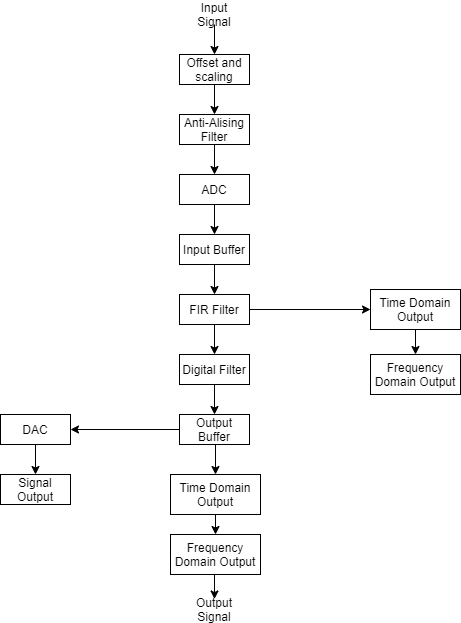
\includegraphics[width=0.6\linewidth]{Images/extra/SystemOverview.png}
%     \caption{Flow of the entire filtering process \cite{preprac2} (adaption)}
%      \label{fig:Transversal}
% \end{figure}

% \pendsign

% \section[2021/05/02]{Sunday, 2 May 2021}

% \subsection{Components From Previous Designs}\label{D:PreviousWork}
% This ESP 411 Practical 2 assignment includes a continuation on work already done in a previous ESP 411 Practical 1 assignment. The practical guide states that the manner in which the input signal is obtained and digitized for this practical can be the same as that used in Practical 1. Therefore, the students are allowed to implement some of their previous designs and work, in this practical implementation. The designs thus used from the previous practical include that of the offset and scaling circuit, the anti-aliasing filter and the Fast Fourier Transform (FFT). The designs and implementation for these circuits and code can be found in the technical report for that practical \cite{ESP_Report1}. This group's Practical 1 technical report can be used as a guide to confirm some statements made in this section.

% \subsection{Filter Design}\label{D:Filter}
% Using the Window method a low-pass FIR is to be designed, using the following cut-off frequency ($f_c$) as the pass-band frequency ($f_p$), the stop-band frequency ($f_s$), stop-band attenuation ($A_s$) and sampling frequency ($F_s$) specifications.
% \vspace{-3mm}
% \begin{align}
%     F_s &= 51.2kHz \\
%     f_p &= 1.5kHz \\
%     f_s &= 3kHz \\
%     A_s &> 50dB
% \end{align}
% Thus the transition width ($\Delta f$) is calculated as:
% \begin{align}
%     \Delta f(f_s - f_p) &= 1.5kHz
% \end{align}

% Since the Windowing method is to be used to calculate the coefficients of the digital filter's impulse response, the frequency specifications of the target filter characteristics, needs to be normalised relative to the sampling frequency. The normalised specifications are thus:
% \vspace{-2mm}
% \begin{align}
%     F_{s\_norm} &= 1 \\
%     f_{p\_norm} &= 0.029296875 \\
%     f_{s\_norm} &= 0.05859375 \\
%     \Delta f &= 0.02936875 \label{eq:Normalised Transition Width}\\
%     w_c &= 2\pi\cdot f_{p\_norm} = 0.1840776945 \\
%     A_s &> 50dB
% \end{align}



% When the Window method is to be used to calculate the coefficients, the starting point of the design is an ideal low-pass frequency response as illustrated in Figure \ref{fig:LPF}, where the cut-off frequency and frequency scale is normalised to $T=1$:

% \begin{figure}[H]
%     \centering
%     \includegraphics[scale=0.5]{Images/Theoretical Background/windowing 1.JPG}
%     \caption{Normalised ideal low-pass filter response}
%     \label{fig:LPF}
% \end{figure}

% The time-domain equivalent of the ideal frequency response in Fig. \ref{fig:LPF} is a sinc function as derived in Eq. \ref{FIR_1} and Eq. \ref{FIR_2}. Thus, to realise the rectangular, low-pass frequency response (illustrated in Fig. \ref{fig:LPF}), a signal that exists for all time ($t \in (-\infty,\infty)$) is required in the time domain.
% The ideal impulse response ($h_D(n)$) for a low-pass filter:
% \begin{align}
%     f_D(n) &=
%     \begin{cases}
%         2 f_p \frac{sin(n\omega_p)}{n\omega_p} & \text{if $n \neq 0$,}\\
%         2 f_p & n=0
%     \end{cases}
%     \label{eq:ideal impulse response for a low-pass filter}
% \end{align}
% With
% \begin{align}
%     \omega_p &= 2\pi f_p
% \end{align}

% However, as discussed in Sec. \ref{TB:The Windowing Method}, this impulse response can not be practically implemented. To overcome this problem, the ideal impulse response in Eq. \ref{eq:ideal impulse response for a low-pass filter} is truncated, by multiplying it with a suitable windowing function that would ensure the resulting filter approximates the ideal impulse response to a degree such that the filter satisfy its requirements.

% For this application of a digital filter, the most important aspect of the specifications is the minimum stopband attenuation that needs to be achieved. Since the minimum stopband attenuation is 50dB ($A_s > 50dB$) and considering the maximum stopband attenuation achievable by the general windowing functions in Table \ref{tb:window functions table}, the Blackman windowing function was chosen to implement the digital filter.

% The set of time-domain points of the impulse response of the filter (the filter's coefficients) can then be calculated as:

% \vspace{-3mm}
% \begin{equation}
%     h(n) = h_D(n) \cdot w(n)
%     \label{eq:ideal impulse response times windowing function}
% \end{equation}

% The Blackman windowing function can be expressed as: \cite{ESP411}

% \begin{equation}
%     w(n) = 0.42 + \frac{1}{2} cos(\frac{2\pi n}{N-1}) + 0.08 cos(\frac{2\pi n}{N-1}) \text{, with $|n| \leq \frac{N-1}{2} $}
%     \label{eq:blackman windowing function}
% \end{equation}

% To counteract the smearing effect of the window function on the filter response, the cut-off frequency used will be centered on the transition band:
% \vspace{-2.5mm}
% \begin{align}
%     f'_c &= f_c + \frac{\Delta f}{2} \\
%     &= 1.5 + 0.75 \\
%     f'_c &= 2.25kHz \\
%     f'_c\_norm &= 0.028125 \\
%     f_p &= f'_c
% \end{align}

% Using the Blackman windowing function, Eq. \ref{eq:ideal impulse response times windowing function} can be expanded into:

% \begin{equation}
%     h(n) = 
%     \begin{cases}
%         2 f_p \frac{sin(n\omega_p)}{n\omega_p} \times [0.42 + \frac{1}{2} cos(\frac{2\pi n}{N-1}) + 0.08 cos(\frac{2\pi n}{N-1})] & \text{if $n \neq 0$} \\
%         2 f_p \times [0.42 + \frac{1}{2} cos(\frac{2\pi n}{N-1}) + 0.08 cos(\frac{2\pi n}{N-1})] & \text{if $n=0$}
%     \end{cases}
%     \nonumber
%     \label{eq:windowing function filter impulse response equation}
% \end{equation}

% in the above equation $N$ is number of coefficients required to implement the filter (based on the transition width and sampling frequency) and $n$ is the coefficient index. 

% %The number of coefficients required to implement a Blackman filter is given as: \cite{ESP411}
% The required normalised transition width is related to the number of coefficients required to implement a Blackman filter by: \cite{ESP411}

% \begin{equation}
%     \Delta f = \frac{5.5}{N}
%     \label{eq:detla f and num coefficients}
% \end{equation}

% Using Eq. \ref{eq:detla f and num coefficients} and the required normalised transition width, Eq. \ref{eq:Normalised Transition Width}, the number of coefficients required to implement the digital filter when sampling at a frequency of $F_s = 51.2kHz$ can be calculated as:

% \vspace{-9mm}
% \begin{align}
%     N &= \frac{5.5}{\Delta f} \nonumber \\
%     N &= \frac{5.5}{0.029296875} \nonumber \\
%     N &= 187.7\overline{3}
% \end{align}

% To ensure odd, positive symmetry, $N$ is rounded up to the next odd number. Thus $N$ is chosen to be 189. The coefficients of $h(n)$ was calculated using a python script (contained in Appendix A) by applying Eq. \ref{eq:ideal impulse response times windowing function} with $-\frac{N-1}{2} < n < \frac{N-1}{2} \text{, }n \in \mathbb{Z}$. The resulting frequency response of the filter, $H(z)$ can be obtained by performing a Fast Fourier Transform (FFT) on the calculated filter impulse response, $h(n)$.

% The impulse response, scaled by the Blackman windowing function, was simulated and the FFT was performed on the impulse response to obtain the frequency response of the designed filer, the results of these simulations is contained in the next section and was used to ensure correct operation.

% In order to implement the digital filter, as designed in this section, on the STM32F45K22 Discovery Board and reduce the number of calculations required, the filter coefficients is calculated at system startup and stored in a lookup table for later reference. The implementation on the embedded platform is discussed in the next section.

% \newpage
% \subsection{STM32 Software Implementation} \label{STM32_Software_Implementation}

% This section describes the manner in which the STM32F45K22i Discovery Board was configured in order to implement the correct frequency sampling and digital filter (as discussed above) as well as display the resulting input and output signal's time-domain and frequency domain response (FFT) on its display. The HAL (Hardware Abstraction Layer) libraries was used to control and interact with the microcontroller’s hardware and thus to implement this practical on the STM32 Discovery board.

% \subsubsection{Timer and ADC sampling rate}
% Timer 2 (TIM2) on the STM32 board was used to trigger an Analogue to Digital Converter (ADC) conversion at the required sampling rate. To achieve this, the APB2 prescaler was configured to generate an APB1 peripheral clock (PCLK1) with frequency 42 MHz. Timer 2 is driven by the APB1 peripheral clock. Thus, in order to acquire an clock signal with frequency of $F_s = 51200 \text{ kHz}$, the period of the Timer 1 module needs to be correctly configured. The amount of times the sampling frequency can divide into the PCLK1's frequency:

% \begin{equation}
%     N_{div} = \frac{42000 \text{ kHz}}{51.2 \text{ kHz}} = 820.2125
% \end{equation}

% Thus, configuring the TIM2 period to 820, a sampling rate of 51 200 Hz can be closely approximated. The time period between successive TIM2 generated signal cycles is thus:

% \begin{equation}
%     T_{TIM2} = \frac{1}{42 \text{ MHz}} \cdot 820 = 19.5238 us
% \end{equation}

% Resulting in an a frequency of:

% \begin{equation}
%     F_{TIM2} = \frac{1}{19.5238us} = 51219.51 Hz
% \end{equation}

% Which is close to the required sampling frequency of 51200 Hz.The ADC was configured to sample at a higher frequency to ensure sampling completion before the next sample starts. The ADC clock prescaler was set to 2, thus the clock-rate used for all ADC operations were half that of the APB2 peripheral clock bus (84 MHz).

% % The various Window functions is discussed in section \ref{TB:The Windowing Method}. The Blackman is chosen, with the following parameters:
% % \begin{table}[H]
% %     \centering
% %     \caption{Design parameters of the Blackman window function}
% %     \begin{tabular}{ |c|c|c|c|c| } 
% %     \hline
% %     Transition width ($Hz$) & Pass-band ripple & Main lobe vs  & $A_s$ & Window function\\ 
% %     (Normalised) & ($dB$) & side lobe ($dB$) & ($dB$) & $w(n), |n| \leq (N-1)/2$ \\
% %     \hline
% %     $\frac{5.5}{N}$ & 0.0017 & 57 & 75 & $0.42+0.5cos(\frac{2\pi n}{N - 1})+$\\
% %     & & & & $0.08cos(\frac{4\pi n}{N-1})$ \\
% %     \hline
% %     \end{tabular}
% %     \label{table:BMParameters}
% % \end{table}


% \section[2021/05/03]{Monday, 3 May 2021}

% The FIR is implemented in Python to simulate the filter response. The coefficients were calculated using the ideal impulse response and the Blackman window function as designed in section \ref{D:Filter}. The coefficients are plotted in Figure \ref{fig:FIRPlot}a and the resulting frequency response in Figure \ref{fig:FIRPlot}b, using the built-in FFT function of the numpy library.

% \begin{figure}[H] 
% \centering
% \captionsetup{justification=centering}
%   \subfloat[Impulse response coefficients, $h(n)$]{% 
%     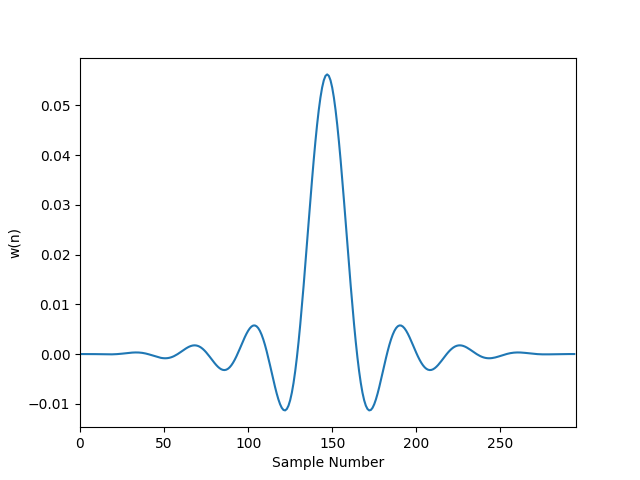
\includegraphics[width=0.48\textwidth]{Images/Simulation/impulseDigitalFilter.png} 
%   } 
%   \hfill 
%   \subfloat[Frequency response of FIR filter, $H(f)$]{% 
%     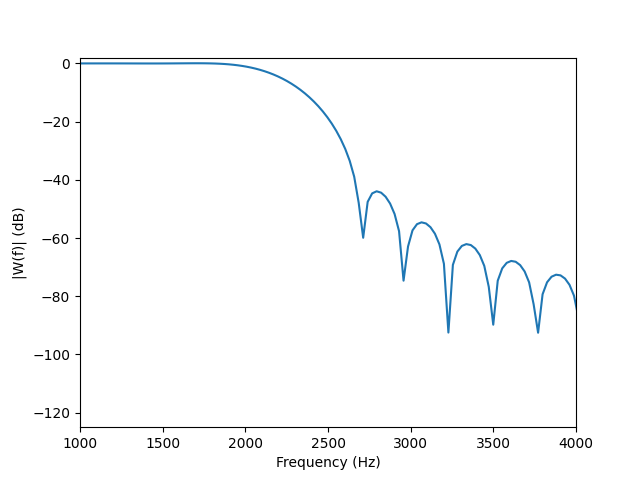
\includegraphics[width=0.48\textwidth]{Images/Simulation/frequencyDigitalFilter.png} 
%   } 
%   \caption{Responses of the Blackman window function.} 
%   \label{fig:FIRPlot}
% \end{figure}

% \subsection{Frequency Response}\label{subsect:frequency_response}
% The FIR low-pass filter is simulated at frequencies of $1kHz$, $1.5kHz$ ($f_c$), $3kHz$ ($f_s$) and $5kHz$, as seen in Figures (\ref{fig:1kFreq} - \ref{fig:5kFreq})a and the output frequency responses in Figures (\ref{fig:1kFreq} - \ref{fig:5kFreq})b are achieved:
% \begin{figure}[H] 
% \centering
% \captionsetup{justification=centering}
%   \subfloat[Sinusoidal wave input]{% 
%     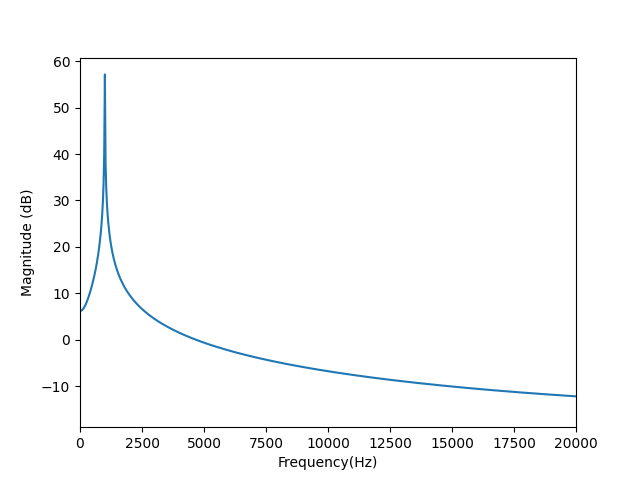
\includegraphics[width=0.48\textwidth]{Images/Simulation/frequencySinusoid1k.png} 
%   } 
%   \hfill 
%   \subfloat[Output from FIR.]{% 
%     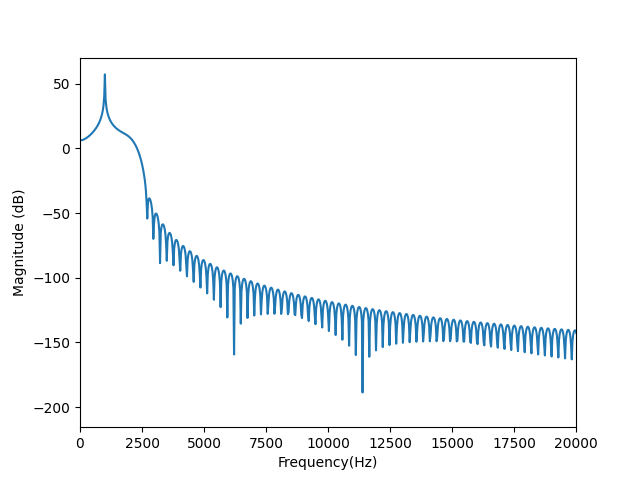
\includegraphics[width=0.48\textwidth]{Images/Simulation/frequencyDigitalFilter1k.png} 
%   } 
%   \caption{Frequency response of the FIR at $1kHz$.} 
%   \label{fig:1kFreq}
% \end{figure}
% At frequencies $1kHz$ (Figure \ref{fig:1kFreq}) and $1.5kHz$  (Figure \ref{fig:1kFreq}) minimal degradation of the signal's output compared to the input magnitude is observed, with a large reduction in noise at frequencies larger than the stop-band frequency.
% \begin{figure}[H] 
% \centering
% \captionsetup{justification=centering}
%   \subfloat[Sinusoidal wave input]{% 
%     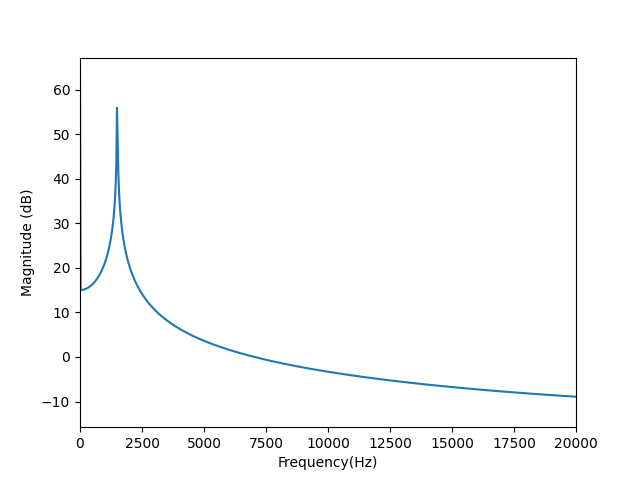
\includegraphics[width=0.48\textwidth]{Images/Simulation/frequencySinusoid1k5.png} 
%   } 
%   \hfill 
%   \subfloat[Output from FIR.]{% 
%     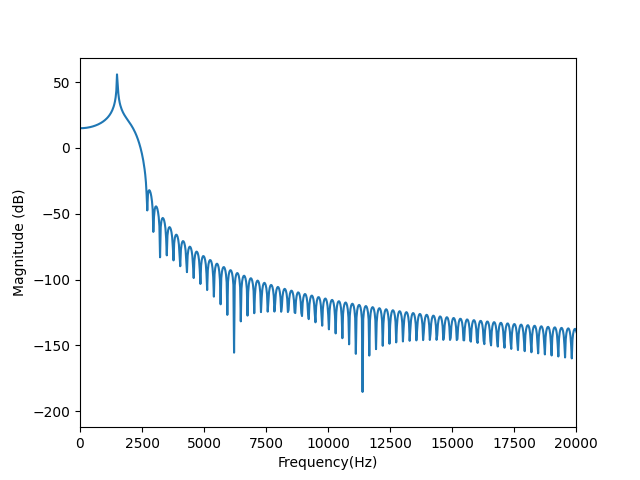
\includegraphics[width=0.48\textwidth]{Images/Simulation/frequencyDigitalFilter1k5.png} 
%   } 
%   \caption{Frequency response of the FIR at $1.5kHz$.} 
%   \label{fig:1k5Freq}
% \end{figure}
% In Figure \ref{fig:3kFreq}, it is seen that at the input frequency of $3kHz$, the output signal's magnitude is greatly reduced from over $50dB$ to just under $0dB$ at the $3kHz$ frequency. The same result can be observed in Figure \ref{fig:5kFreq} with a greater difference between the input and output magnitudes.
% \begin{figure}[H] 
% \centering
% \captionsetup{justification=centering}
%   \subfloat[Sinusoidal wave input]{% 
%     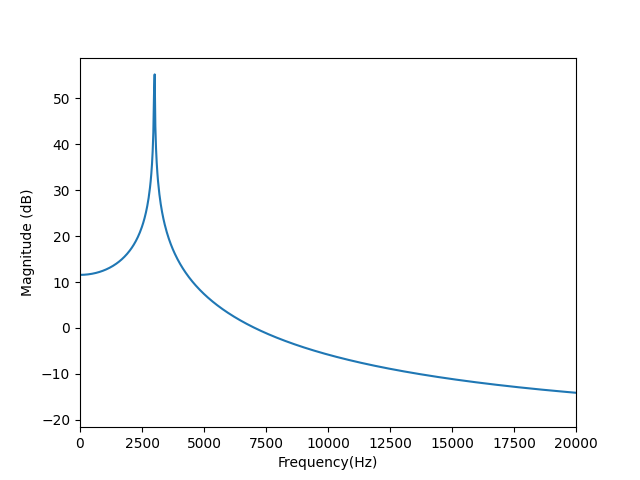
\includegraphics[width=0.48\textwidth]{Images/Simulation/frequencySinusoid3k.png} 
%   } 
%   \hfill 
%   \subfloat[Output from FIR.]{% 
%     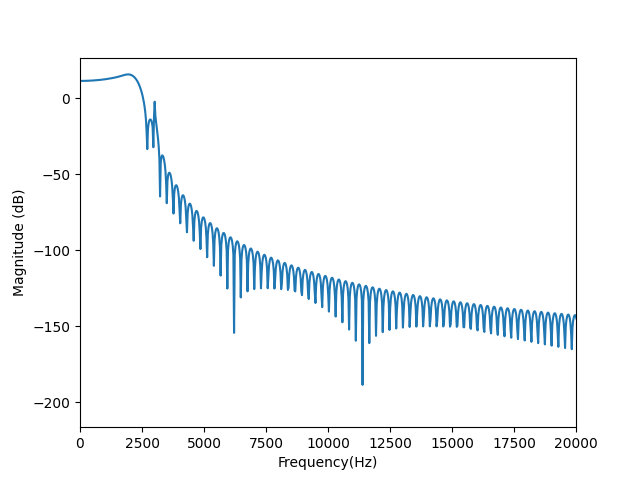
\includegraphics[width=0.48\textwidth]{Images/Simulation/frequencyDigitalFilter3k.png} 
%   } 
%   \caption{Frequency response of the FIR at $3kHz$.} 
%   \label{fig:3kFreq}
% \end{figure}

% \begin{figure}[H] 
% \centering
% \captionsetup{justification=centering}
%   \subfloat[Sinusoidal wave input]{% 
%     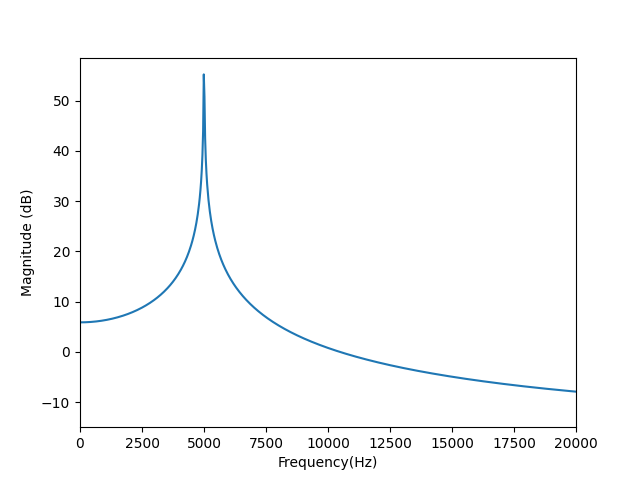
\includegraphics[width=0.48\textwidth]{Images/Simulation/frequencySinusoid5k.png} 
%   } 
%   \hfill 
%   \subfloat[Output from FIR.]{% 
%     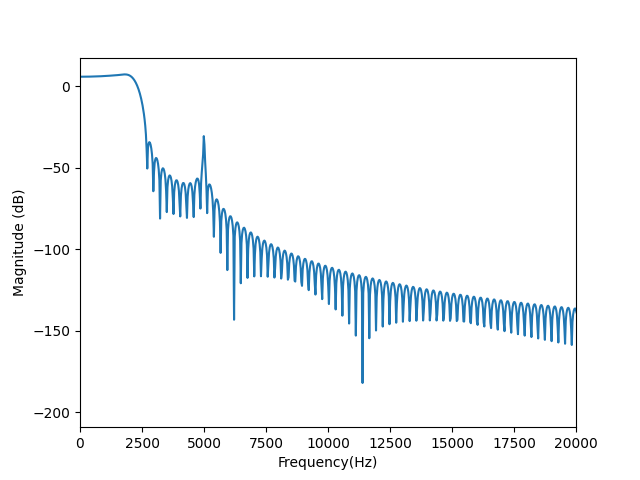
\includegraphics[width=0.48\textwidth]{Images/Simulation/frequencyDigitalFilter5k.png} 
%   } 
%   \caption{Frequency response of the FIR at $5kHz$.} 
%   \label{fig:5kFreq}
% \end{figure}

% \subsection{Transient Response}\label{sect:transient_response}
% The FIR low-pass filter is simulated at frequencies of $1kHz$, $1.5kHz$ ($f_c$), $3kHz$ ($f_s$) and $5kHz$. Minimal reduction in amplitude of the signal at $1kHz$, Figure \ref{fig:1kSig}. There is a greater reduction in amplitude of the signal at $1.5kHz$ at later stages, but an increase for the first period. For Figure \ref{fig:3kSig} and \ref{fig:1k5Sig}, the magnitudes are greatly reduced and within 4 periods completely.
% \begin{figure}[H] 
% \centering
% \captionsetup{justification=centering}
%   \subfloat[Sinusoidal wave input]{% 
%     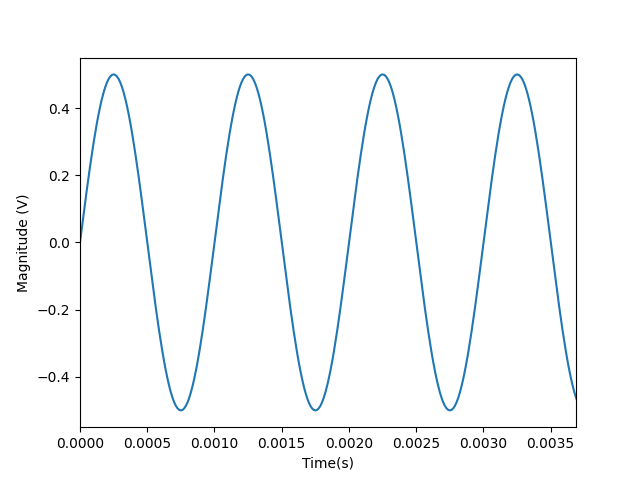
\includegraphics[width=0.48\textwidth]{Images/Simulation/timeSinusoid1k.png} 
%   } 
%   \hfill 
%   \subfloat[Output from FIR.]{% 
%     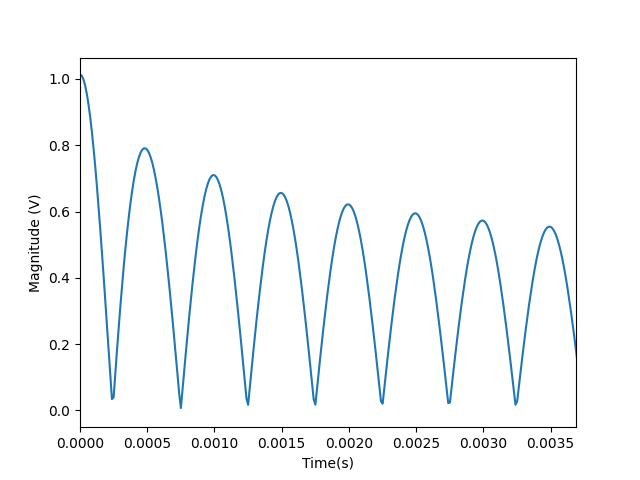
\includegraphics[width=0.48\textwidth]{Images/Simulation/timeDigitalFilter1k.png} 
%   } 
%   \caption{Transient response of the FIR at $1kHz$.} 
%   \label{fig:1kSig}
% \end{figure}

% \begin{figure}[H] 
% \centering
% \captionsetup{justification=centering}
%   \subfloat[Sinusoidal wave input]{% 
%     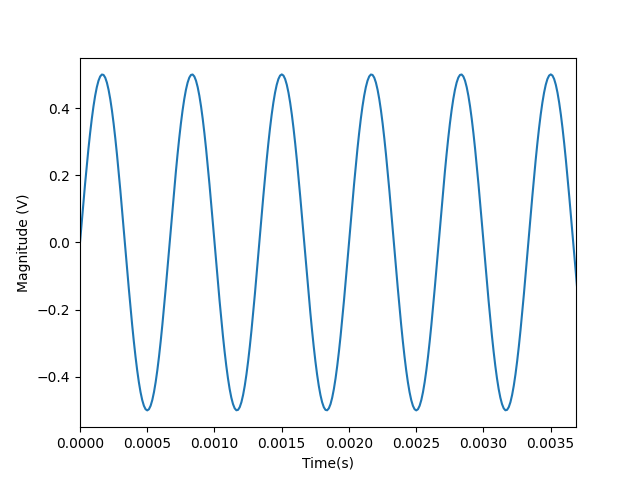
\includegraphics[width=0.48\textwidth]{Images/Simulation/timeSinusoid1k5.png} 
%   } 
%   \hfill 
%   \subfloat[Output from FIR.]{% 
%     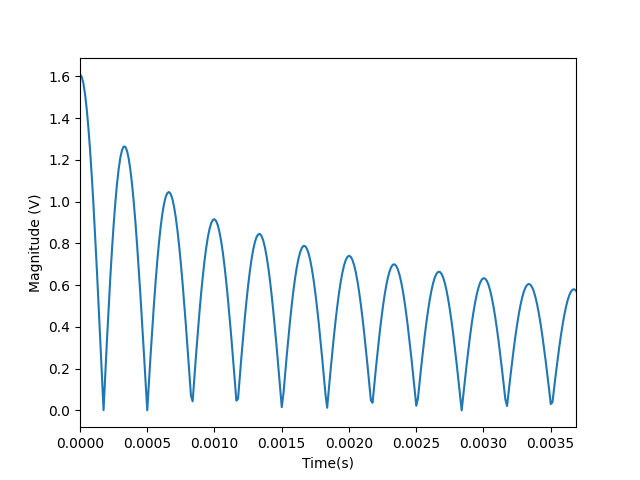
\includegraphics[width=0.48\textwidth]{Images/Simulation/timeDigitalFilter1k5.png} 
%   } 
%   \caption{Transient response of the FIR at $1.5kHz$.} 
%   \label{fig:1k5Sig}
% \end{figure}

% \begin{figure}[H] 
% \centering
% \captionsetup{justification=centering}
%   \subfloat[Sinusoidal wave input]{% 
%     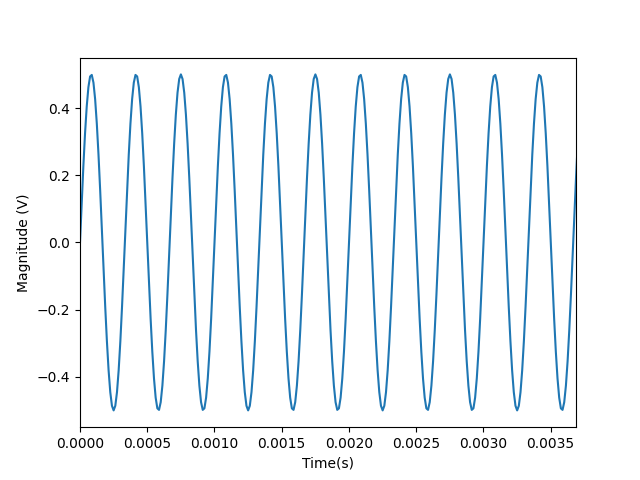
\includegraphics[width=0.48\textwidth]{Images/Simulation/timeSinusoid3k.png} 
%   } 
%   \hfill 
%   \subfloat[Output from FIR.]{% 
%     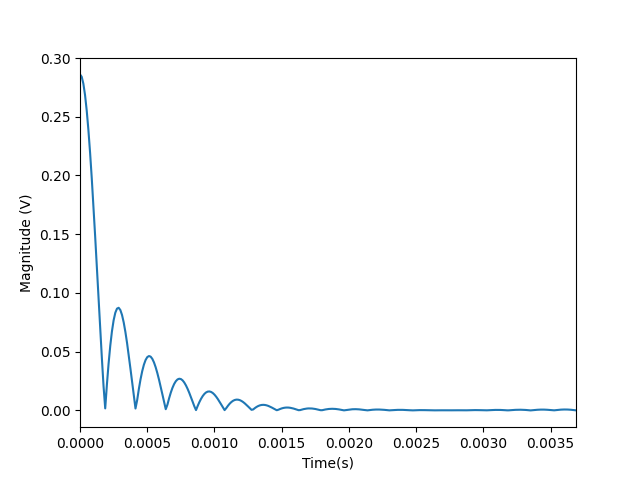
\includegraphics[width=0.48\textwidth]{Images/Simulation/timeDigitalFilter3k.png} 
%   } 
%   \caption{Transient response of the FIR at $3kHz$.} 
%   \label{fig:3kSig}
% \end{figure}

% \begin{figure}[H] 
% \centering
% \captionsetup{justification=centering}
%   \subfloat[Sinusoidal wave input]{% 
%     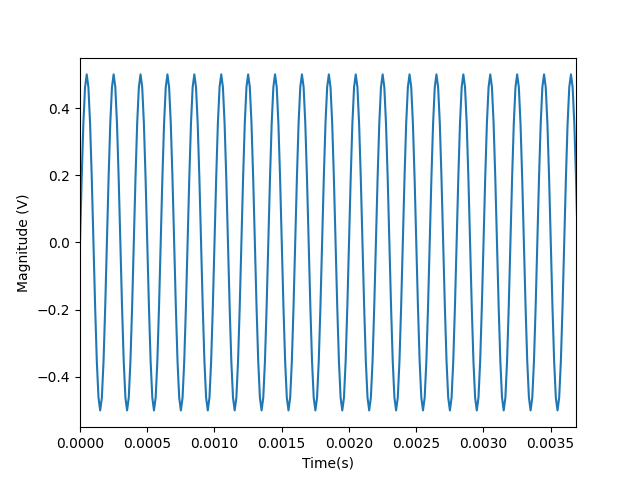
\includegraphics[width=0.48\textwidth]{Images/Simulation/timeSinusoid5k.png} 
%   } 
%   \hfill 
%   \subfloat[Output from FIR.]{% 
%     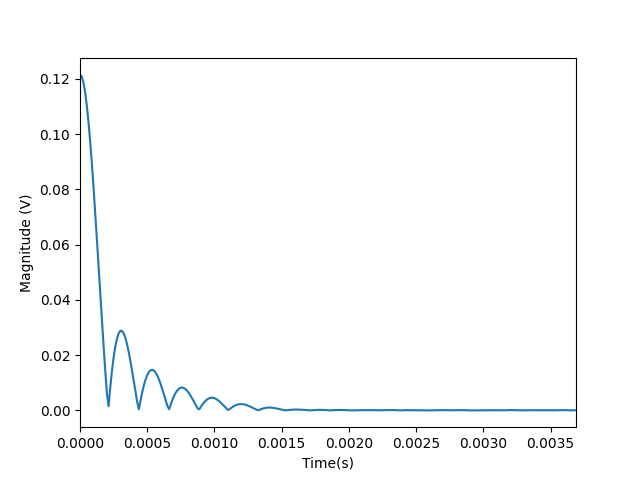
\includegraphics[width=0.48\textwidth]{Images/Simulation/timeDigitalFilter5k.png} 
%   } 
%   \caption{Transient response of the FIR at $5kHz$.} 
%   \label{fig:5kSig}
% \end{figure}

% The experiment is conducted in the following manner. One thing to note is the lack of oscilloscopes and wave generators. This is so, because at the time of writing this report,  getting access to labs with this equipment was not easy.

% \begin{figure}[H]
%     \centering
%     \captionsetup{justification=centering}
%     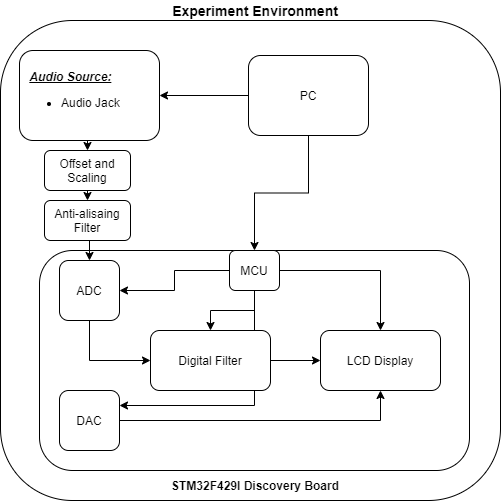
\includegraphics[width=0.8\linewidth]{Images/extra/experiment.png}
%     \caption{Experimental Setup}
%      \label{fig:Experiment}
% \end{figure}

% The experimental setup shows all the components that play a part in successfully demonstrating what is happening in the system. The setup shows that the audio source that will be used for the system comes from the audio jack port on a PC. The same PC is used to program the STM32 Discovery board so that it can implement the digital filter as well as display etc. The setup also shows that an offset and scaling as well as a anti-aliasing filter is implemented. These analogue circuits and filters are used to get the sampled signal in the correct ranges for the ADC to function properly, as well as filter out any aliasing that might occur during the sampling. The setup also shows a LCD display. The LCD display will be used to show all the needed information about the system, to illustrate that everything is functioning as intended. The setup lastly show the implementation of a DAC. The DAC will be used to transform the sampled and filtered signal back into a continuous line signal that will demonstrate the affects sampling and filtering have on the original signal.

% \subsection{Python Implementation of Digital Filter}

% \lstinputlisting[breaklines]{Code/Simulasies.py}


% \pendsign

% \section[2021/05/14]{Friday, 14 May 2021}

% The results displayed below are obtained by sampling an audio signal produced by a smartphone via an audio jack. The audio signal is processed and sampled as was done in practical 1 \cite{ESP_Report1}. The results below show four different sets of obtained results. The first set of plots show the time and frequency domain output of the input signal. The second set of plots show time and frequency domain plots of the output signal after digital filtering. Each set consist of the results of sinusoidal input signals at $1kHz$, $1.5kHz$, $3kHz$ and $5kHz$.

% \subsection{Input Signal}\label{subsect:resultsinput}
% The input signal's time and frequency response plots, plotted on the STM32F429-Discovery Board are shown below.
% \subsubsection{Time Domain}\label{subsect:resultsinputtime}
% The input signals' amplitudes are $0.6V$ and the plot range from $0V$ to $3.6V$. The time axis is divided into bins of $97.5\mu s$ and a range of $2.535ms$
% \begin{figure}[H] 
% \centering
% \captionsetup{justification=centering}
%   \subfloat[$1kHz$ sinusoidal wave input]{% 
%     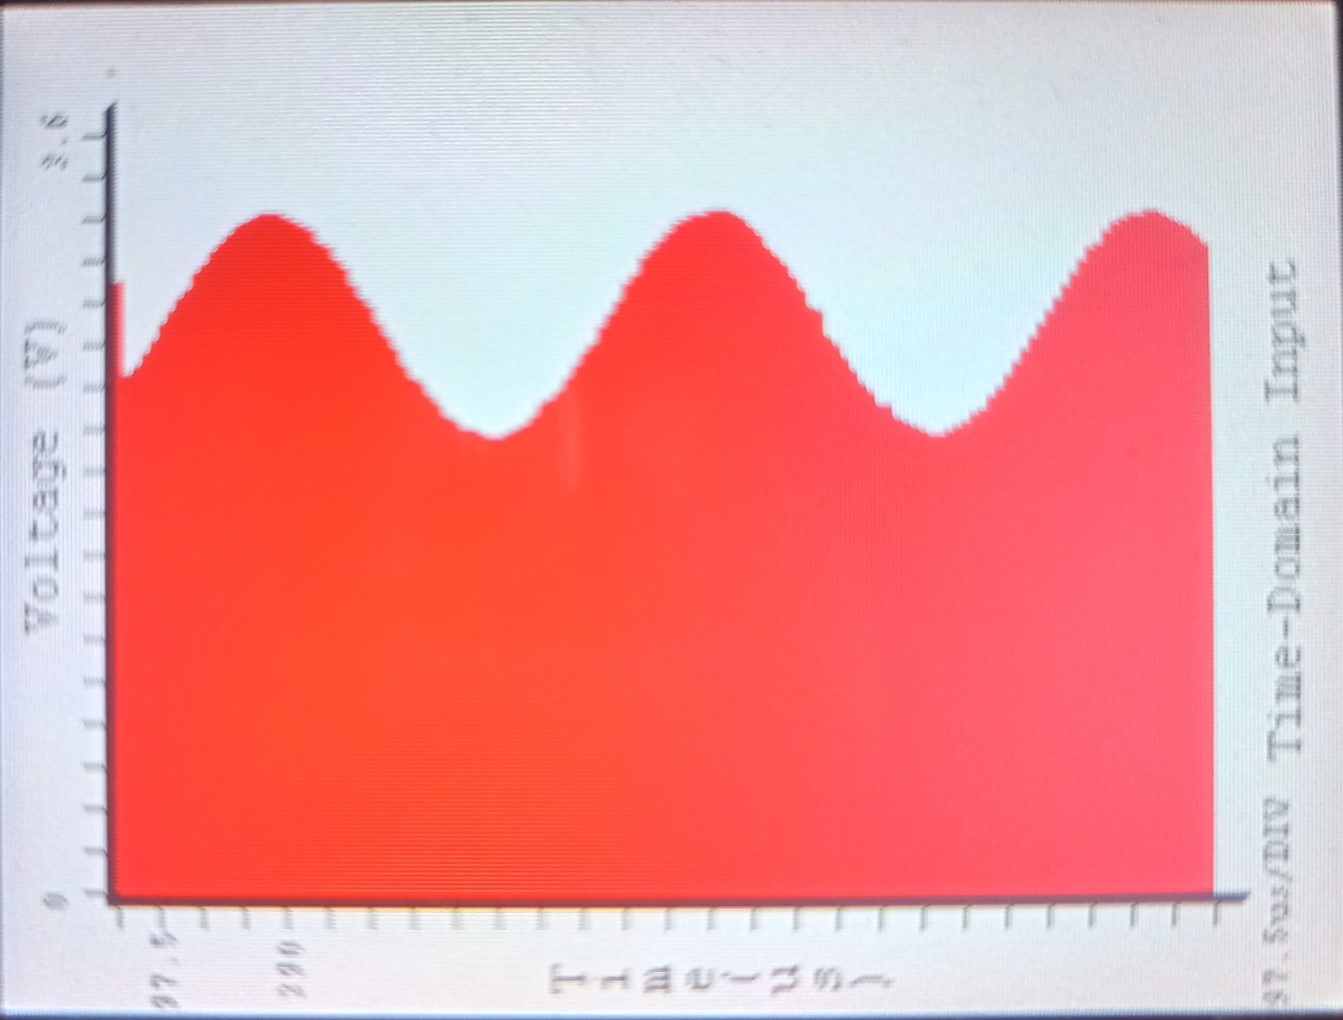
\includegraphics[width=0.45\textwidth]{Images/Results/inputTime1k.jpg} 
%   }\quad
%   \subfloat[$1.5kHz$ sinusoidal wave input]{% 
%     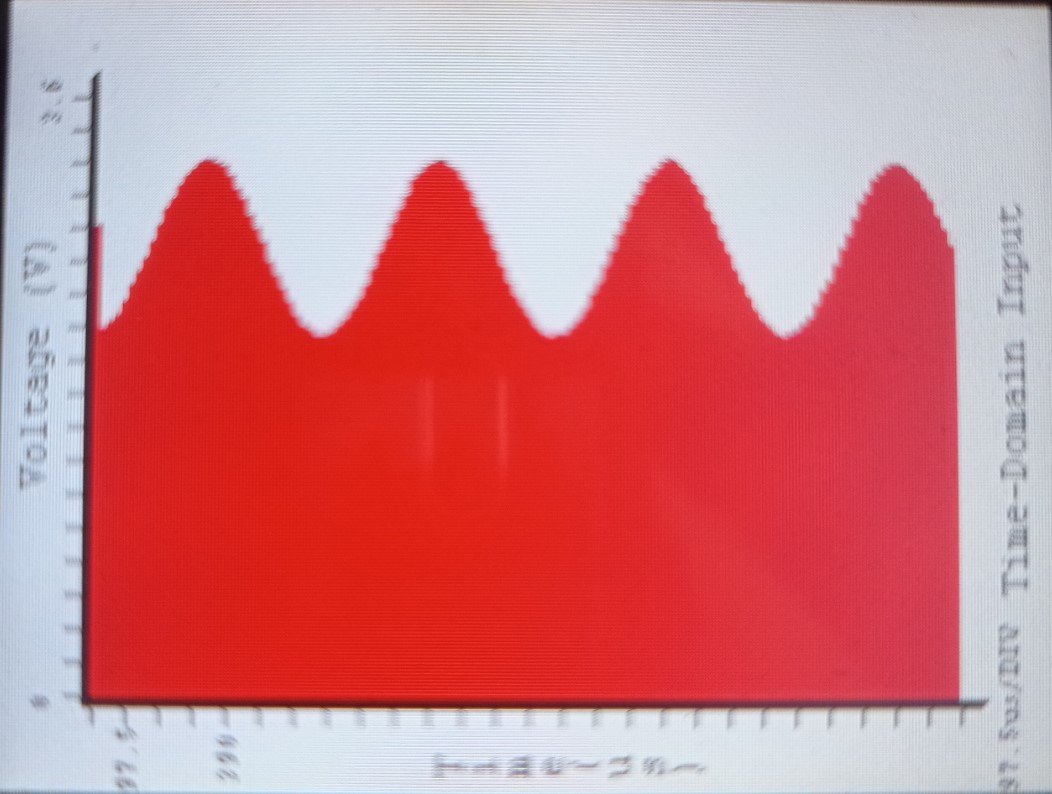
\includegraphics[width=0.45\textwidth]{Images/Results/inputTime1k5.jpg} 
%   } 
%   \caption{Input signals in the time domain.} 
%   \label{fig:inputsignalsTimeD1}
% \end{figure}
% \begin{figure}[H] 
% \centering
% \captionsetup{justification=centering}
%     \subfloat[$3kHz$ sinusoidal wave input]{% 
%     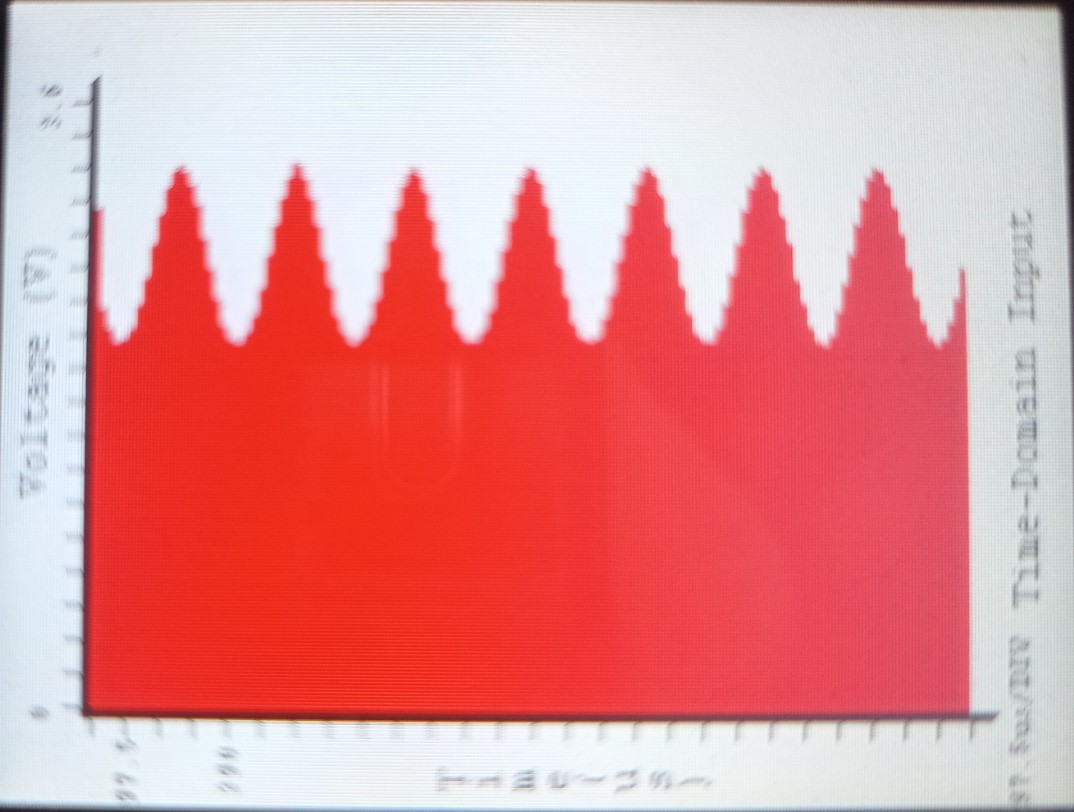
\includegraphics[width=0.45\textwidth]{Images/Results/inputTime3k.jpg} 
%   } 
%   \quad
%   \subfloat[$5kHz$ sinusoidal wave input]{% 
%     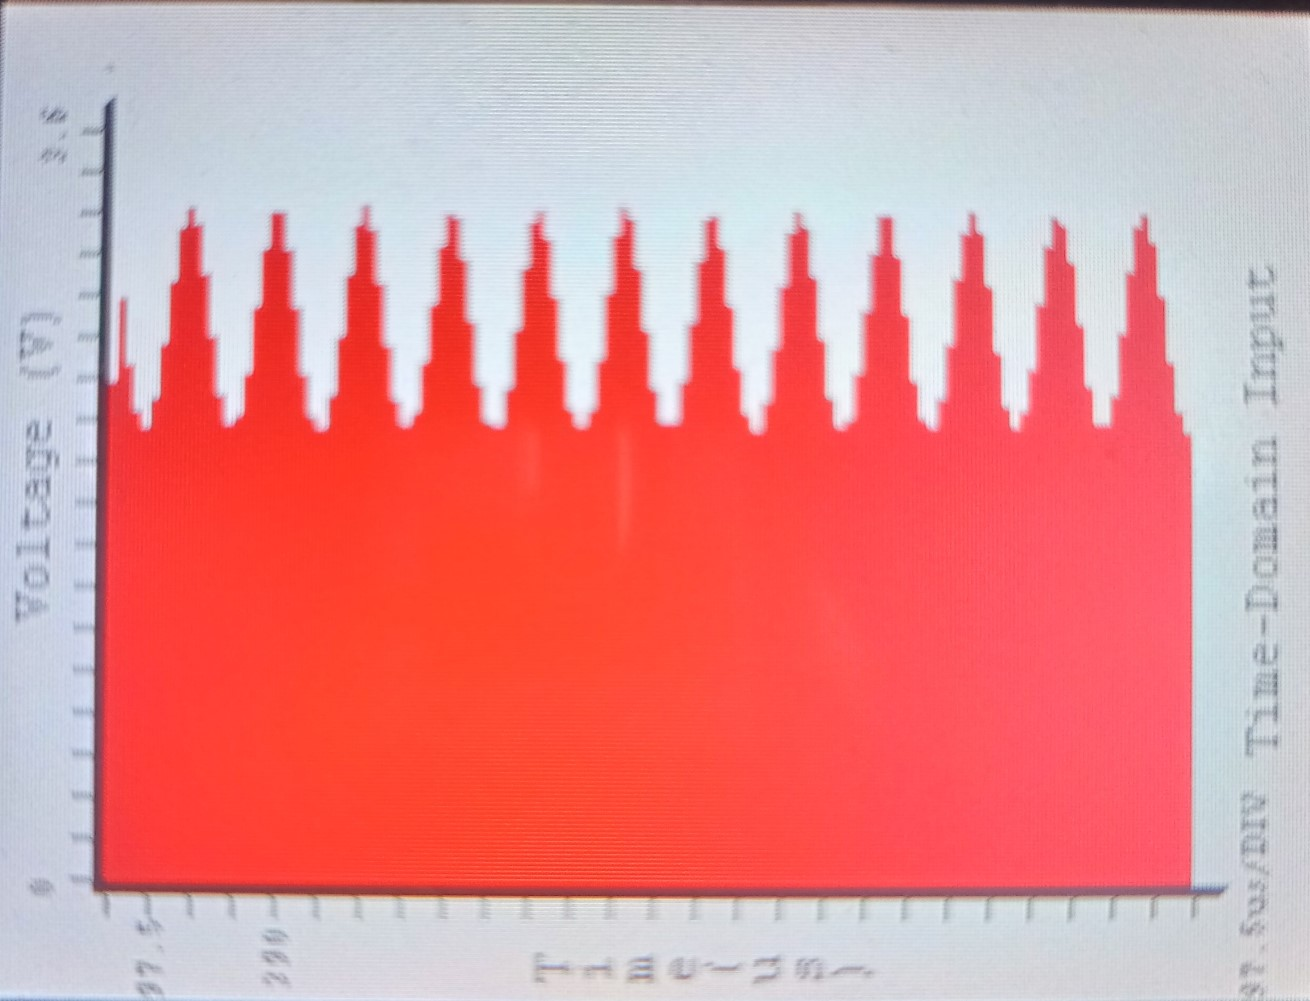
\includegraphics[width=0.45\textwidth]{Images/Results/inputTime5k.jpg} 
%   } 
%   \caption{Input signals in the time domain.} 
%   \label{fig:inputsignalsTimeD2}
% \end{figure}


% \subsubsection{Frequency Domain}\label{subsect:resultsinputfrequency}
% The input signals after the FFT operation. The response is shown between 0 and $20kHz$, with bins of $200Hz$. The response is normalised to the main harmonic, with noise mostly between $-30dB$ and $-50dB$.
% \begin{figure}[H] 
% \centering
% \captionsetup{justification=centering}
%   \subfloat[Frequency response at $1kHz$ input signal]{% 
%     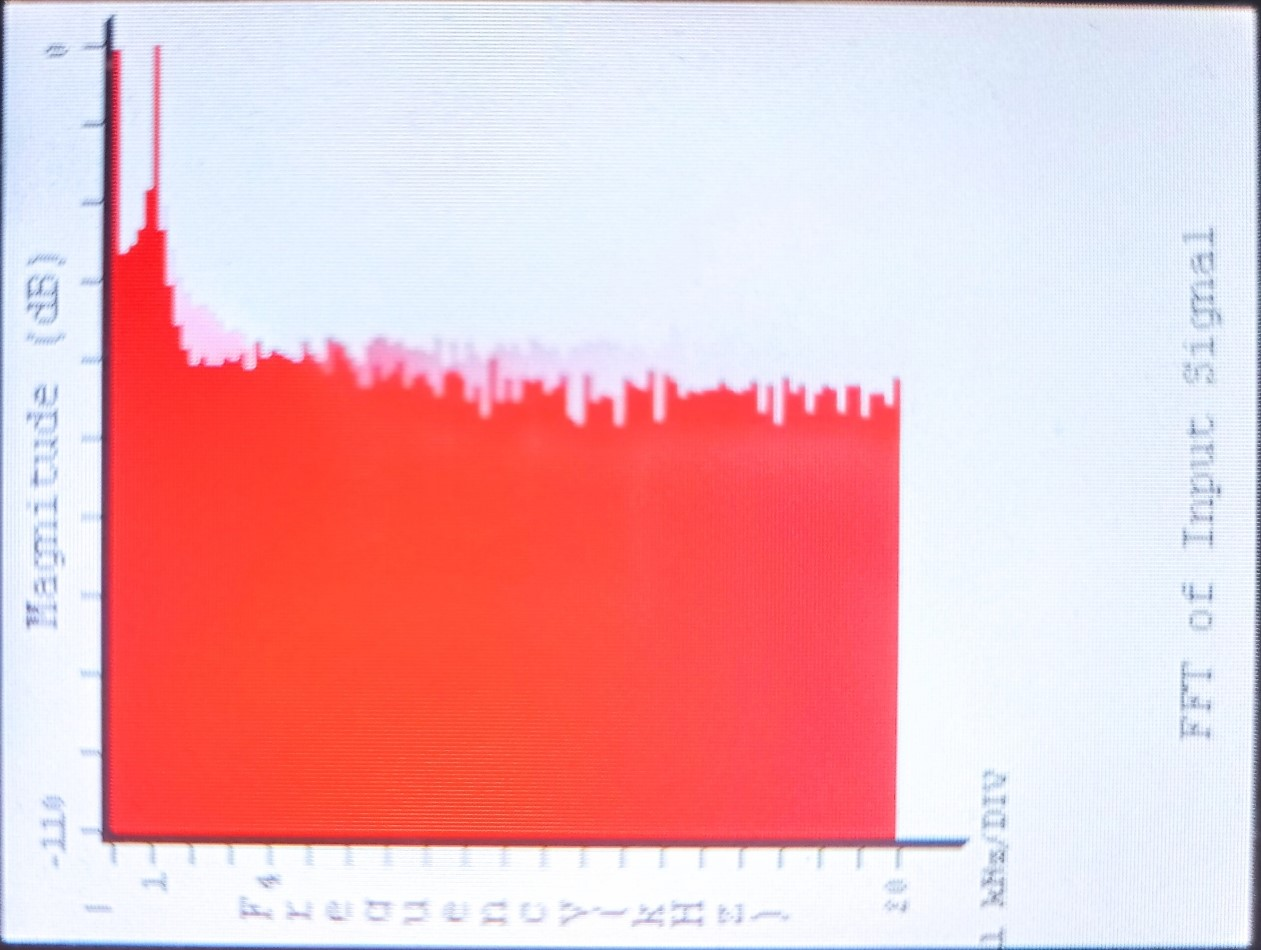
\includegraphics[width=0.45\textwidth]{Images/Results/inputFreq1k.jpg} 
%   } 
%   \quad 
%   \subfloat[Frequency response at $1.5kHz$ input signal]{% 
%     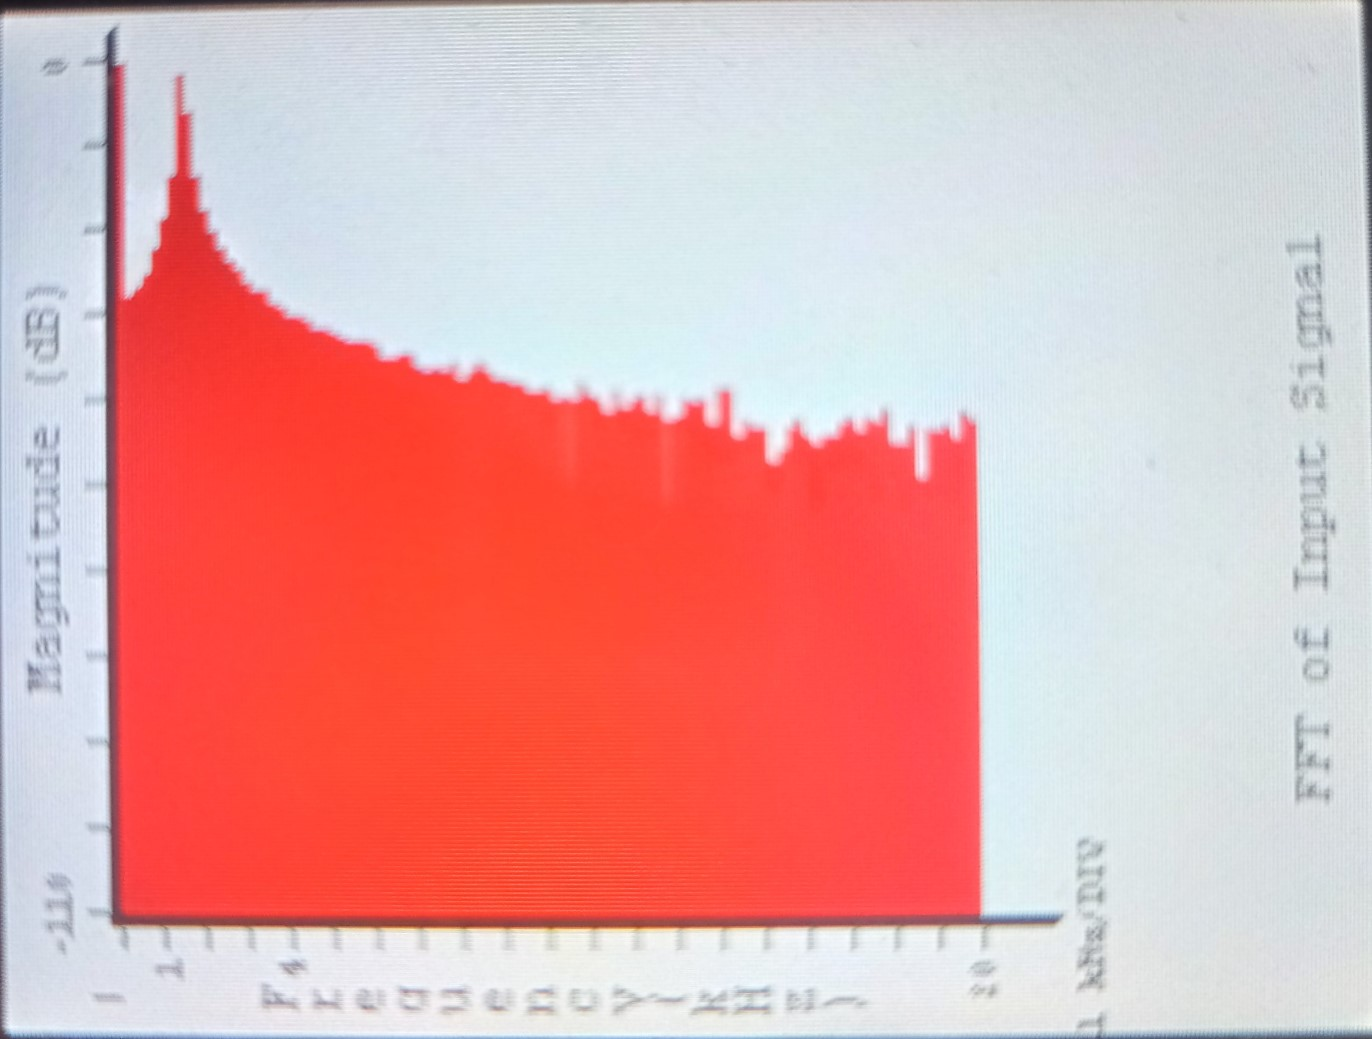
\includegraphics[width=0.45\textwidth]{Images/Results/inputFreq1k5.jpg} 
%   } 
%   \caption{Input signals in the frequency domain.} 
%   \label{fig:inputsignalFreq1}
% \end{figure}

% \begin{figure}[H] 
% \centering
% \captionsetup{justification=centering}
%     \subfloat[Frequency response at $3kHz$ input signal]{% 
%     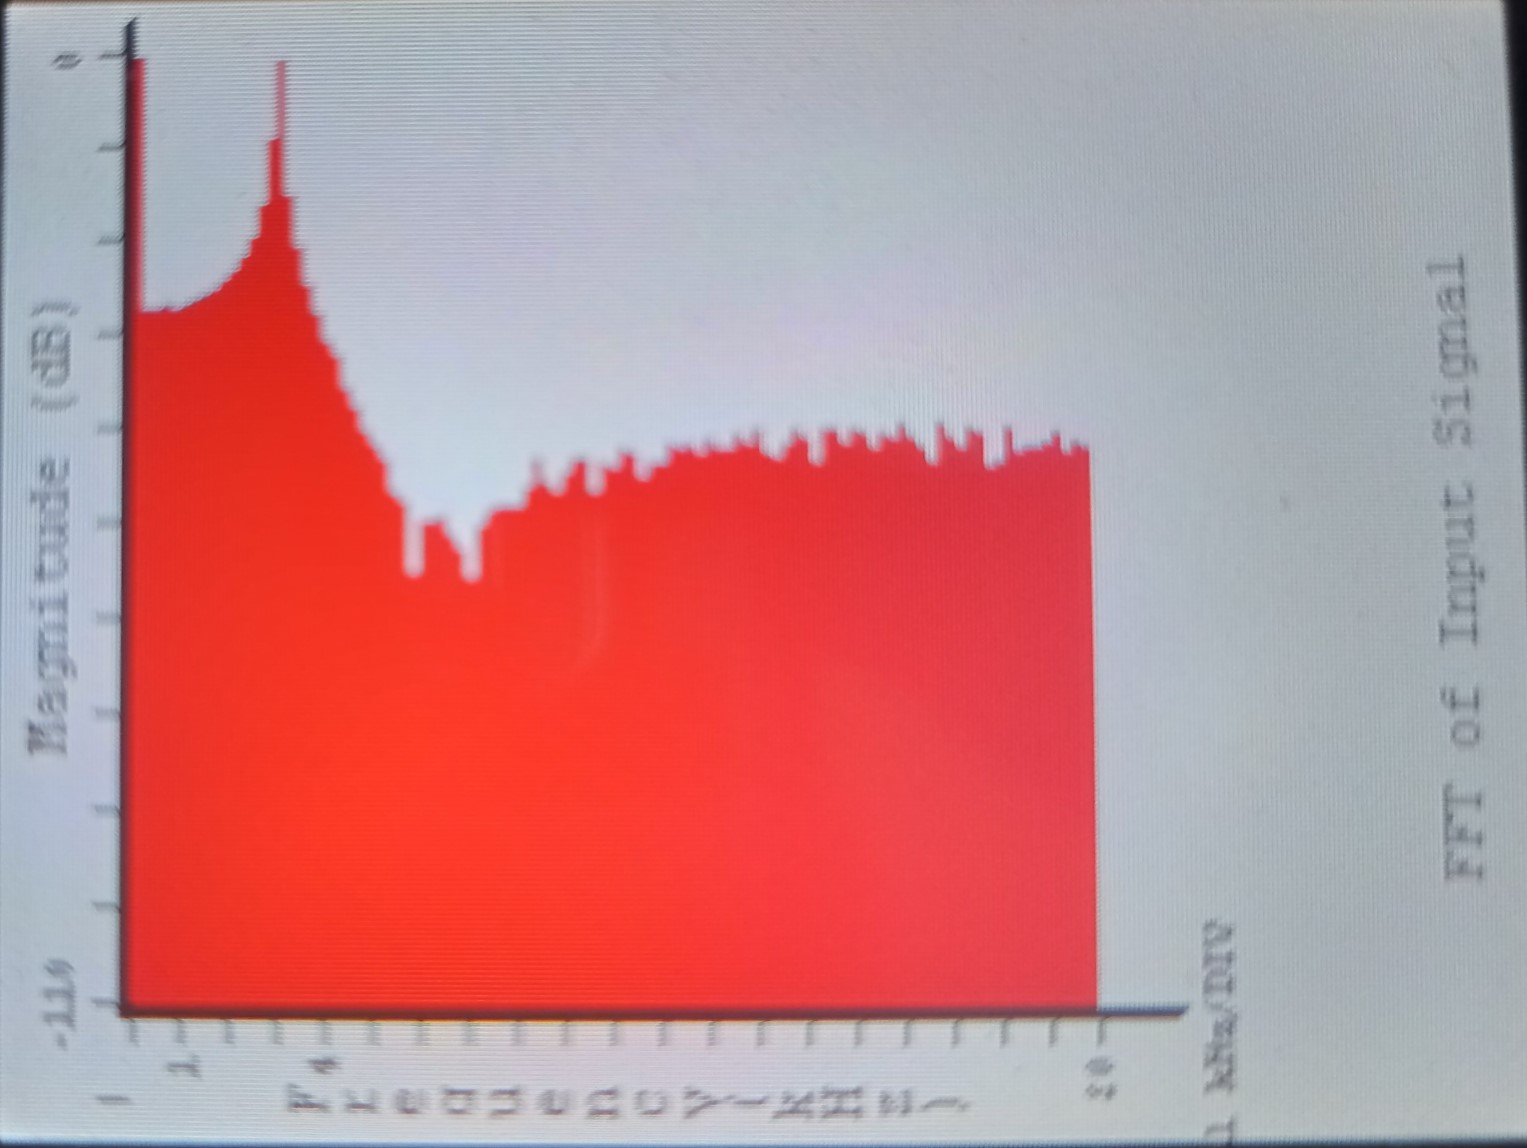
\includegraphics[width=0.45\textwidth]{Images/Results/inputFreq3k.jpg} 
%   }
%   \quad 
%   \subfloat[Frequency response at $5kHz$ input signal]{% 
%     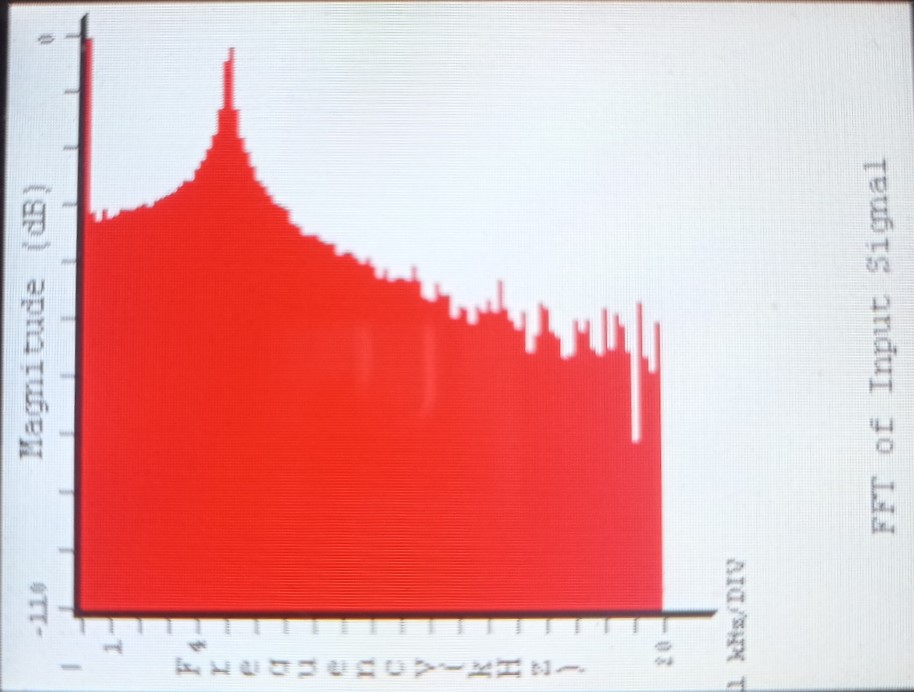
\includegraphics[width=0.45\textwidth]{Images/Results/inputFreq5k.jpg} 
%   } 
%   \caption{Input signals in the frequency domain.} 
%   \label{fig:inputsignalFreq2}
% \end{figure}
% \newpage
% \subsection{Output Signal}\label{subsect:resultsoutput}
% The output signal's time and frequency response plots, plotted on the STM32F429-Discovery Board are shown below.
% \subsubsection{Time Domain}\label{subsect:resultsoutputtime}
% The axis are set up as in section \ref{subsect:resultsinputtime}. The main difference is the amplitude of the signals, where the amplitude is halved between $1kHz$ and $1.5kHz$ ($f_c$) and no sinusoidal component at the $3kHz$ and $5kHz$ frequencies, as in Figure \ref{fig:outputsignalFreq2}.
% \begin{figure}[H] 
% \centering
% \captionsetup{justification=centering}
%   \subfloat[Filtered sinusoidal wave at $1kHz$]{% 
%     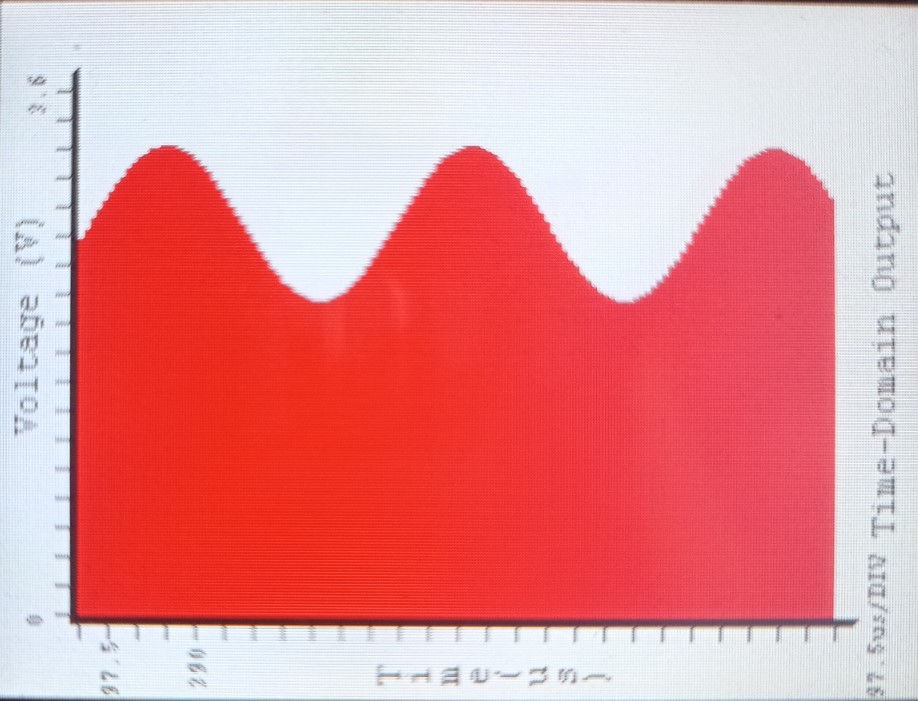
\includegraphics[width=0.45\textwidth]{Images/Results/outputTime1k.jpg} 
%   } 
%   \quad 
%   \subfloat[Filtered sinusoidal wave at $1.5kHz$]{% 
%     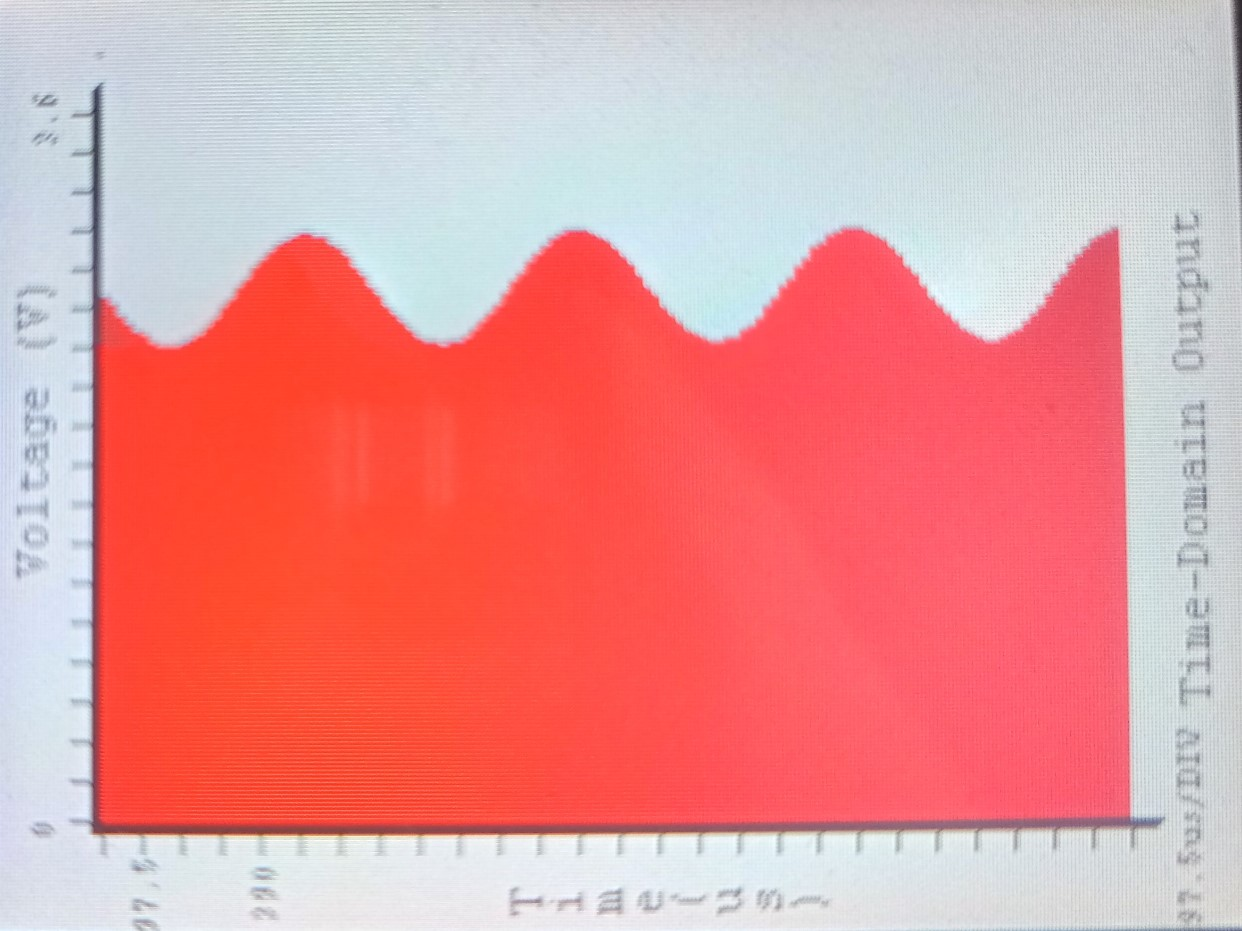
\includegraphics[width=0.45\textwidth]{Images/Results/outputTime1k5.jpg} 
%   } 
%   \caption{Output signal in the time domain} 
%   \label{fig:outputsignalTime1}
% \end{figure}

% \begin{figure}[H] 
% \centering
% \captionsetup{justification=centering}
%   \subfloat[Filtered sinusoidal wave at $3kHz$]{% 
%     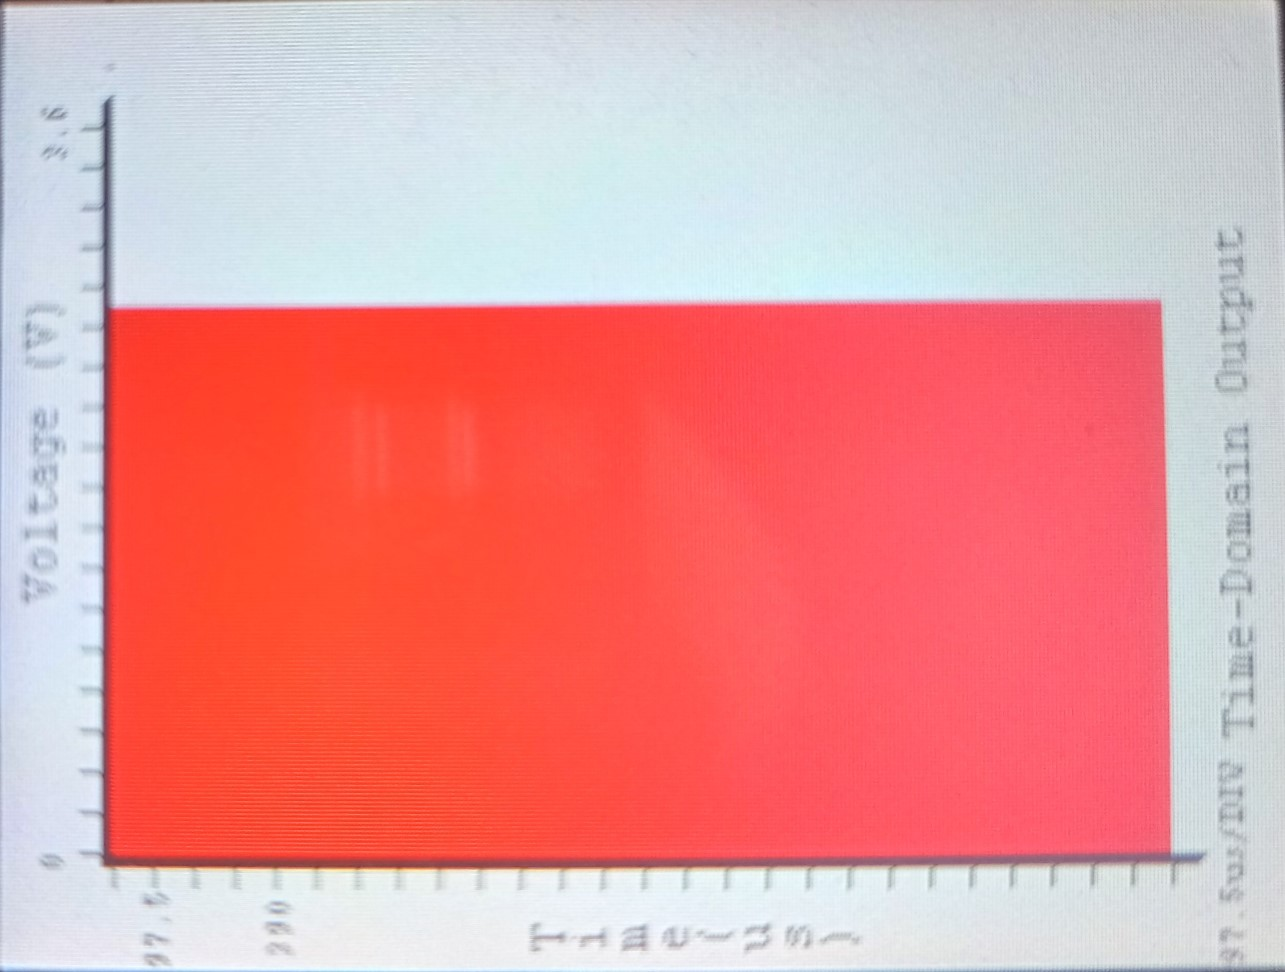
\includegraphics[width=0.45\textwidth]{Images/Results/outputTime3k.jpg} 
%   } 
%   \quad 
%   \subfloat[Filtered sinusoidal wave at $5kHz$]{% 
%     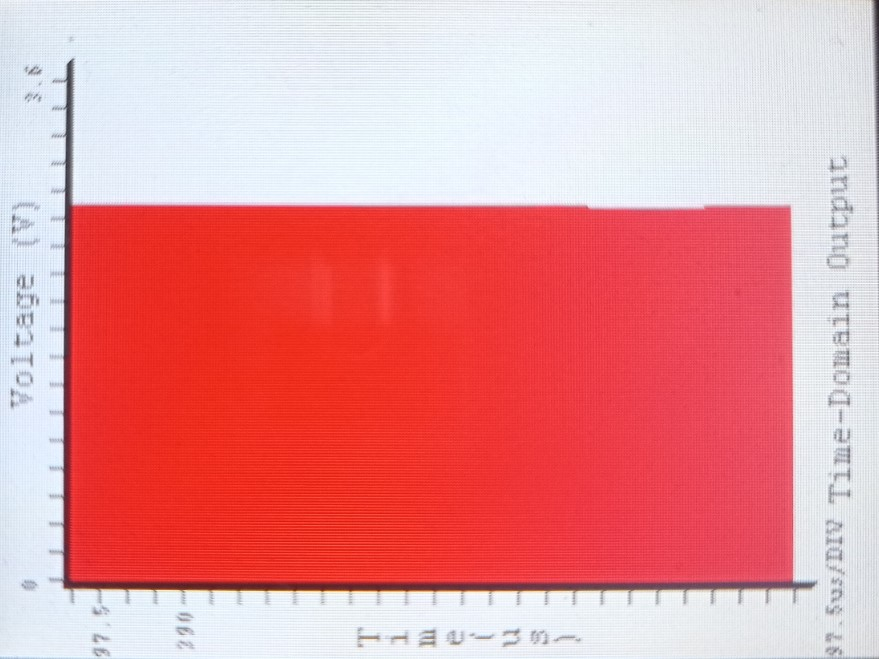
\includegraphics[width=0.45\textwidth]{Images/Results/outputTime5k.jpg} 
%   } 
%   \caption{Output signal in the time domain} 
%   \label{fig:outputsignalTime2}
% \end{figure}

% \newpage
% \subsubsection{Frequency Domain}\label{subsect:resultsoutputfrequency}
% The axis are set up as in section \ref{subsect:resultsinputfrequency}. The FFT is normalised to the input signal's amplitude. The output signal after the transposition procedure is shown. Stable attenuation is seen at $-65dB$ at $1kHz$, only $-50dB$ at $1.5kHz$ and $-100dB$ for $3kHz$ and $5kHz$ frequencies.
% \begin{figure}[H] 
% \centering
% \captionsetup{justification=centering}
%   \subfloat[Filtered frequency response at $1kHz$]{% 
%     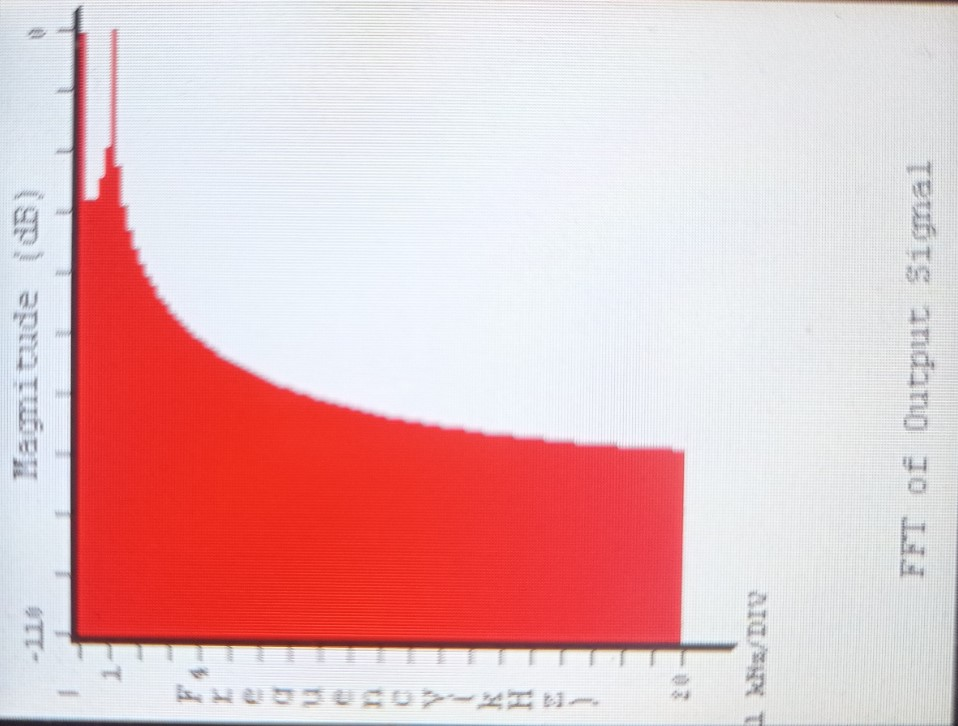
\includegraphics[width=0.45\textwidth]{Images/Results/outputFreq1k.jpg} 
%   } 
%   \quad 
%   \subfloat[Filtered frequency response at $1.5kHz$]{% 
%     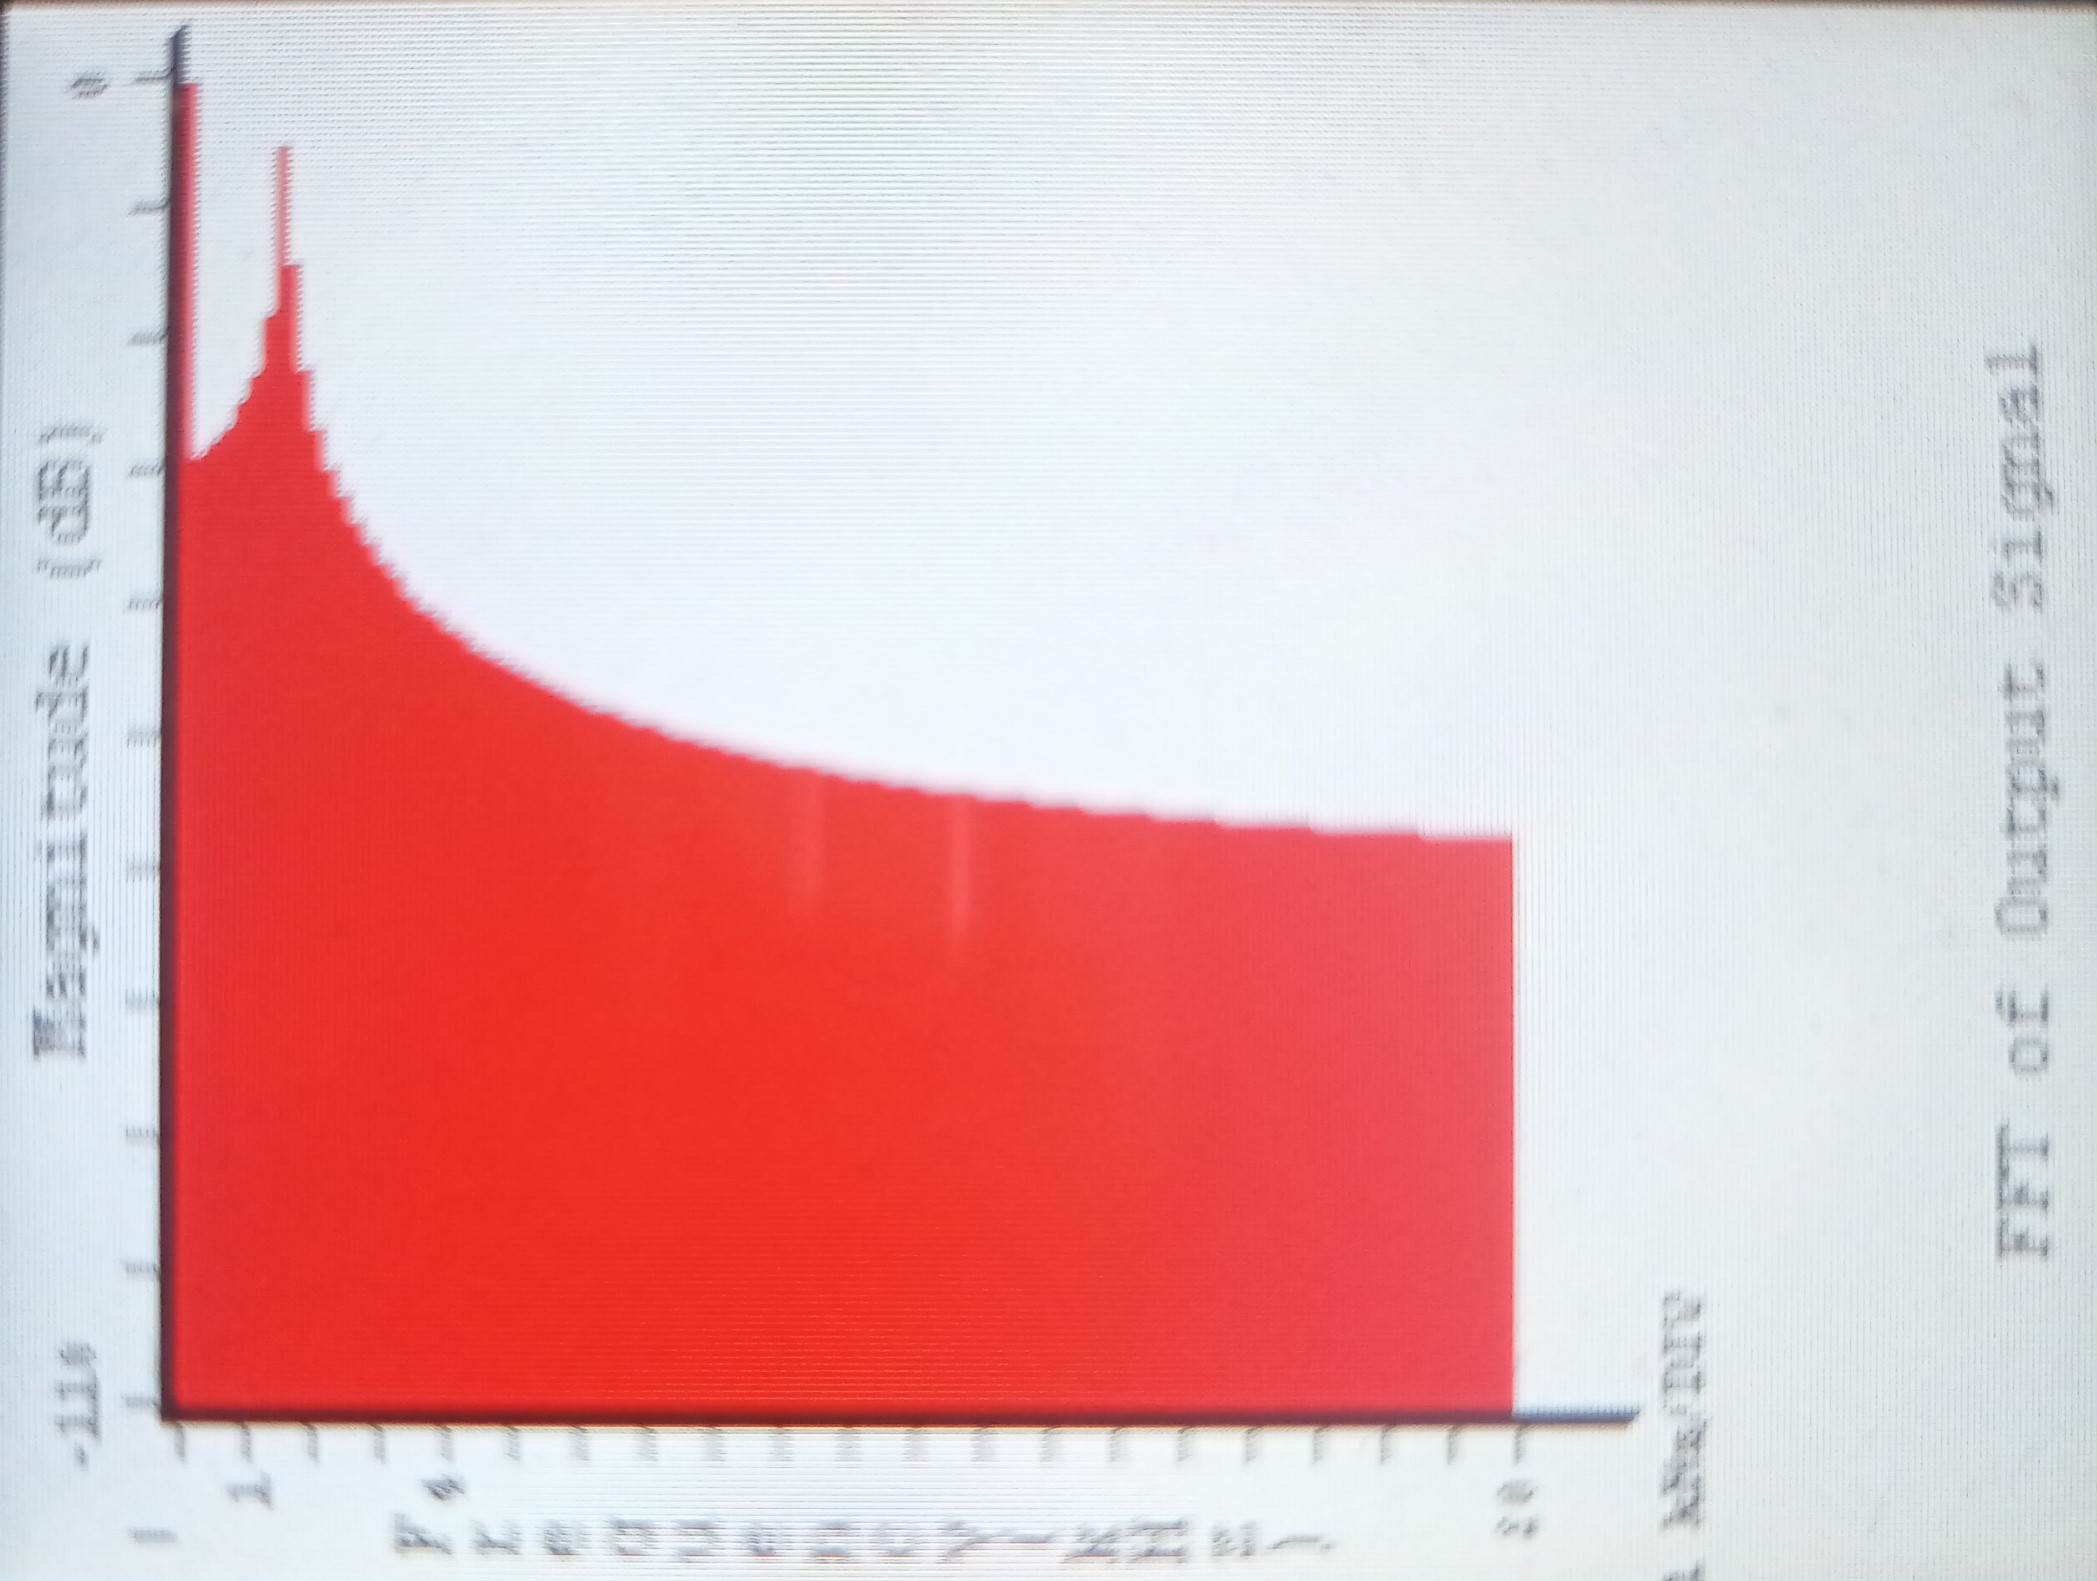
\includegraphics[width=0.45\textwidth]{Images/Results/outputFreq1k5.jpg} 
%   } 
%   \caption{Output signal in the frequency domain.} 
%   \label{fig:outputsignalFreq1}
% \end{figure}

% \begin{figure}[H] 
% \centering
% \captionsetup{justification=centering}
%   \subfloat[Filtered frequency response at $3kHz$]{% 
%     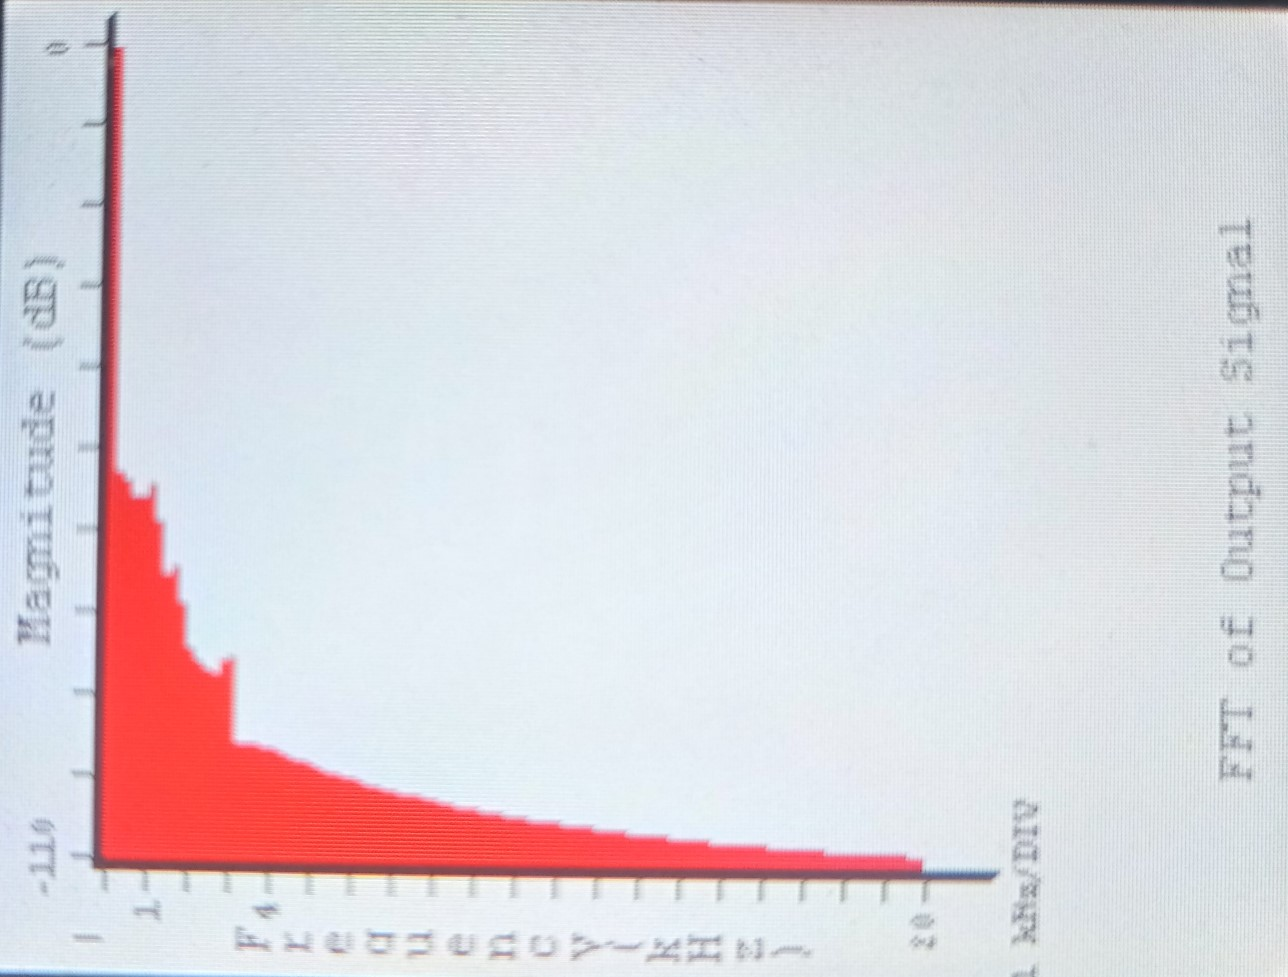
\includegraphics[width=0.45\textwidth]{Images/Results/outputFreq3k.jpg} 
%   } 
%   \quad 
%   \subfloat[Filtered frequency response at $5kHz$]{% 
%     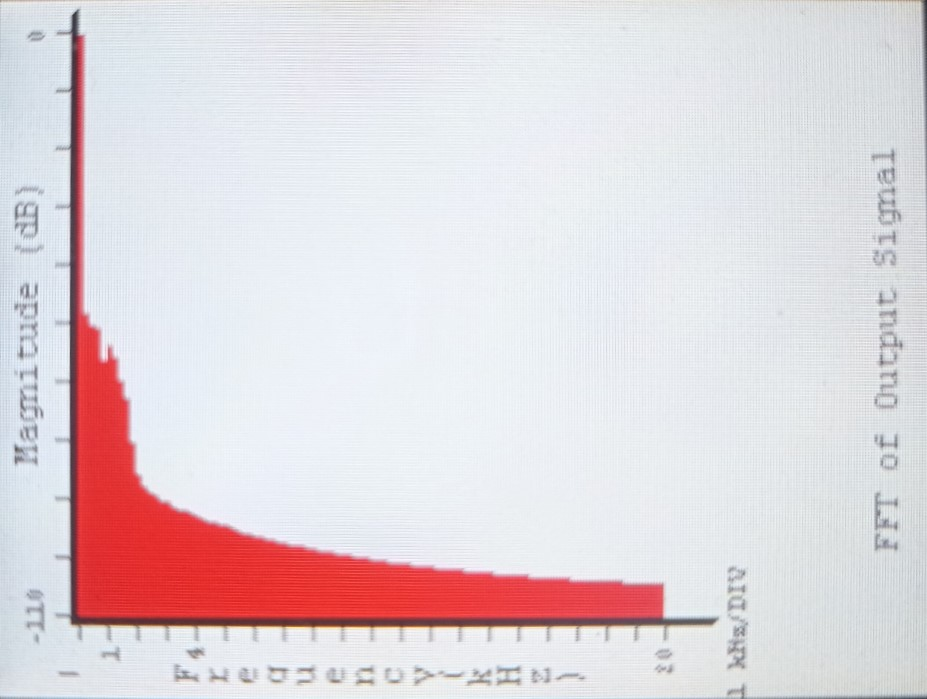
\includegraphics[width=0.45\textwidth]{Images/Results/outputFreq5k.jpg} 
%   } 
%   \caption{Output signal in the frequency domain.}
%   \label{fig:outputsignalFreq2}
% \end{figure}

% \pendsign

% \section[2021/05/25]{Tuesday, 25 May 2021}
% \subsection{Practical 3}
% \begin{itemize}
%     \item Individual design and report
%     \item Focus on design choices
%     \item Start ASAP
%     \item Demo = 3 separate systems combined using best subsystems
%     \item Understand AM frequencies
%     \item Focus on writing down EVERYTHING in lab book
%     \item Theoretical background and literature study important.
% \end{itemize}

% \subsubsection{Broad assignment}
% Each student should design, build and test a unique real-world problem using your knowledge from previous years, as well as experience from Practicals 1 and 2, as basis.
% \begin{itemize}
%     \item You should design an AM channel modelling device to measure and graphically display the channel characteristics of the AM band (526.5 – 1606.5 kHz with 9kHz channel spacing). A minimum resolution of 3 kHz is needed for measurements.
%     \item An anti-aliasing filter should be designed to limit the sampled spectrum to the AM band.
%     \item A user should also be able to select (“digitally tune into”) a specific AM channel. Using digital filtering, a specific AM channel (9 kHz bandwidth) should be filtered out when selected, AM demodulated (digitally) and played out via the DAC output.
%     \item You can use the equipment in the labs to generate an AM signal to use as the input to your designed system. If you do decide to use an antenna, be careful not to use very long wires for them, since it is illegal to broadcast in the AM band without a license.
% \end{itemize}
% \pendsign


\section[2024/05/07]{Tuesday, 7 May 2024}

\href{https://www.mwrcybersec.com/research\_items/juggling-with-tokens-securing-jwts}{JWTs}

% \section[2021/05/25]{Tuesday, 25 May 2021}
% \subsection{Practical 3}
% Subsystems needed for this system:
% \begin{itemize}
%     \item I/O
%     \begin{itemize}
%         \item Display
%         \begin{itemize}
%             \item Graph of entire spectrum
%             \item Graph of certain channel (of 120)
%             \item Axis and intervals in $kHz$ and $dB$
%         \end{itemize}
%         \item AM wave
%         \begin{itemize}
%             \item Colpitts oscillator/Crystal oscillator as carrier
%             \item audio signal multiplied with the carrier
%         \end{itemize}
%         \item Channel selection
%         \begin{itemize}
%             \item Buttons
%             \item Touch screen
%             \item DIP switch
%         \end{itemize}
%         \item Demodulated signal from DAC
%     \end{itemize}
%     \item Full sampling from spectrum
%     \begin{itemize}
%         \item Minimum Frequency resolution of 3kHz 
%         \item $526.5kHz - 1606.5kHz = \Delta 1080kHz$
%         \item make use of all 3 ADCs for fast sampling
%     \end{itemize}
%     \item Single channel sampling
%     \begin{itemize}
%         \item Finer frequency resolution
%         \item Channel width $=9kHz$
%         \item Band-pass filter
%         \item Only use the middle $8kHz$
%         \item $0.5kHz$ guard bands
%         \item Create lookup table for 120 channel filters
%     \end{itemize}
%     \item Build anti-aliasing filter, to cut-off at $>1606.5kHz$
% \end{itemize}
